\chapter{Precoding under Outdated CSI}
\label{chapter:precoding_under_outdated_csi}

% intro
In Chapter~\ref{chapter:mu_mimo_precoding}, linear precoding was developed under the implicit assumption that the \ac{CSI} used to design the precoder coincides with the \ac{CSI} experienced by the \acp{UT} at the moment of transmission.
As discussed in Chapter~\ref{chapter:hts_communication_systems}, this assumption breaks down in the mobile satellite scenario considered in this work, owing to the combination of a large propagation delay and a \ac{UT}-induced Doppler spread.
This chapter is devoted to characterizing the impact of this mismatch on precoder performance and to developing a strategy that compensates for it.

% roadmap
Section~\ref{section:outdated_csi_problem_formulation} formulates the problem precisely and introduces the \ac{CSI} feedback delay as the key operating parameter. From there, the chapter proceeds in three steps.
First, Section~\ref{section:outdated_csi_impact} quantifies the impact of outdated \ac{CSI} on the achievable rate of the linear precoders developed in Chapter~\ref{chapter:mu_mimo_precoding}.
Section~\ref{section:outdated_csi_compensation} then proposes a compensation method that exploits the temporal correlation of the channel in order to predict the instantaneous channel at the time of transmission.
Finally, Section~\ref{section:realistic_channel_evaluation} re-evaluates both the impact of outdated \ac{CSI} and the proposed compensation strategy under a more realistic channel model.

% conclusion
To end this work, the results are applied to a set of representative example scenarios, after which the main findings are summarized in a final conclusion.

\section{Problem Formulation}
\label{section:outdated_csi_problem_formulation}
% ============================
%     Problem Formulation
% ============================

We consider the forward link of the multi-beam \ac{HTS} system as described in Chapter~\ref{chapter:hts_communication_systems}. 
The \ac{GW} serves $K$ \acp{UT} simultaneously through the satellite, equipped with $N_T$ feeds, by applying a linear precoder to the data symbols.
Each \ac{UT} is equipped with $N_R$ receive antennas. The channel of \ac{UT}~$k$ at time $t$ is denoted by $\mathbf{H}_k(t) \in \mathbb{C}^{N_R \times N_T}$ and follows the Rician model from~\eqref{eq:rician_channel_model}.
The received signal at \ac{UT}~$k$ reads
\begin{equation}
\label{eq:outdated_csi_received_signal}
    \mathbf{y}_k(t) = \mathbf{H}_k(t)\;\mathbf{F}(t)\,\mathbf{a}(t) + \mathbf{n}_k(t),
\end{equation}
where $\mathbf{a}(t)$ collects the data symbols of each stream intended for \ac{UT}~$k$ into a column vector, and $\mathbf{n}_k(t) \sim \mathcal{CN}(\mathbf{0}, N_0 \mathbf{I}_{N_R})$ is additive noise.
The precoder satisfies the total transmit-power constraint $\mathrm{tr}\big(\mathbf{F}(t)\mathbf{F}^{\mathsf{H}}(t)\big) \leq P_T$ at any moment in time.

In practice, the channel must first be estimated at the \acp{UT} and fed back to the \ac{GW}, before it can be used to design the precoder.
Denoting the aggregate elapsed time by the \ac{CSI} feedback delay~$\tau_{\mathrm{CSI}}$, the precoder applied at time $t$ is necessarily based on the outdated channel state $\mathbf{H}(t - \tau_{\mathrm{CSI}})$.
How severely this mismatch degrades performance depends on how much the channel has evolved during $\tau_{\mathrm{CSI}}$.

The temporal variability of the channel is characterised through the normalised autocorrelation function of its \ac{NLoS} component, denoted by $R_h(\tau)$.
It is shown in Appendix~\ref{appendix_section:doppler_spectrum} that, under Jakes' model, the autocorrelation between two channel realizations separated by a lag $\tau$ equals the zeroth-order Bessel function of the first kind, evaluated in $2\pi f_D \tau$.
The coherence time of the \ac{NLoS} component is defined as the lag at which the autocorrelation first falls to one half of its peak value:
\begin{equation}
\label{eq:coherence_time_def}
    T_c \;\triangleq\; \max\{\tau > 0 \,:\, R_h(\tau) \geq \frac{1}{2}\}.
\end{equation}

Rather than studying the impact of $\tau_{\mathrm{CSI}}$ in absolute terms, the \ac{CSI} feedback delay is expressed as a fraction of the coherence time throughout the analysis.
Two operating points sharing the same $\tau_{\mathrm{CSI}} / T_c$ exhibit, by construction, the same correlation between the outdated and the instantaneous channel, irrespective of the absolute values of $\tau_{\mathrm{CSI}}$ and $T_c$. 
Reporting results as a function of $\tau_{\mathrm{CSI}} / T_c$ therefore yields conclusions that apply to any combination of carrier frequency, \ac{UT} velocity and orbital altitude consistent with the underlying Rician model.

\section{Impact of Outdated CSI}
\label{section:outdated_csi_impact}
% ==============================
%    Impact of Outdated CSI
% ==============================

% intro
In order to quantify the impact of outdated \ac{CSI} on the system performance, the achievable rate obtained by linear precoders developed in Chapter~\ref{chapter:mu_mimo_precoding} is simulated as a function of the \ac{SNR} for a system in which a \ac{BS} with $8$ transmit antennas serves $4$ \acp{UT} with $2$ receive antennas each.
Each precoder is designed based on the outdated channel state $\mathbf{H}(t - \tau_{\mathrm{CSI}})$ and applied to the instantaneous channel $\mathbf{H}(t)$. The resulting sum rate is averaged over more than $100$ channel realizations, and over multiple coherence periods of the fading process for each realization.
Figures~\ref{fig:impact_outdated_csi_achievable_rate_zf_bd} and~\ref{fig:impact_outdated_csi_achievable_rate_wmmse} report the results for a \ac{CSI} feedback delay $\tau_{\mathrm{CSI}}$ that varies from $0 \, T_c$ (instantaneous \ac{CSI}, used as a reference) up to $5/4\, T_c$, slightly beyond the coherence time.

% general observations
All three precoders are very sensitive to outdated \ac{CSI}. Even a delay of only a quarter of the coherence time causes a substantial loss on the achievable rate at moderate and high \ac{SNR} values. 
The loss with respect to instantaneous \ac{CSI} grows monotonically with $\tau_{\mathrm{CSI}}/T_c$, confirming the intuition that the more outdated the \ac{CSI}, the worse the performance.
Once the \ac{CSI} feedback delay surpasses the coherence time of the \ac{NLoS} component, the system becomes essentially unusable.
This aligns with the definition of $T_c$.
Beyond the point $\tau_{\mathrm{CSI}} \geq T_c$, the channel available at the \ac{GW} and the channel actually experienced by the \acp{UT} are only weakly correlated such that the precoder is in effect designed for a channel that bears little resemblance to the true one.
As a consequence, the precoder fails to exploit the spatial dimension of the channel and the sum-rate collapses.

% ZF and BD
A closer look at Figure~\ref{fig:impact_outdated_csi_achievable_rate_zf_bd} shows that both \ac{ZF} and \ac{BD} precoding saturate at high \ac{SNR} once the \ac{CSI} is even slightly outdated.
Both \ac{ZF} and \ac{BD} precoders completely eliminate the interference between the users, no matter the ratio of the transmit power to the noise power.
With outdated \ac{CSI}, the precoder nulls interference along the wrong directions, leaving a residual inter-user interference that is proportional to the transmit power.
As the \ac{SNR} increases, the system transitions from a noise-limited regime to an interference-limited one and the desired signal and the residual interference grow at the same rate.
Therefore, the \ac{SINR} saturates and the achievable rate converges to a finite ceiling, that is determined solely by the magnitude of the channel evolution over the feedback delay.

\begin{figure}[!htb]
    \centering
    \begin{subfigure}{0.495\textwidth}
        \centering
        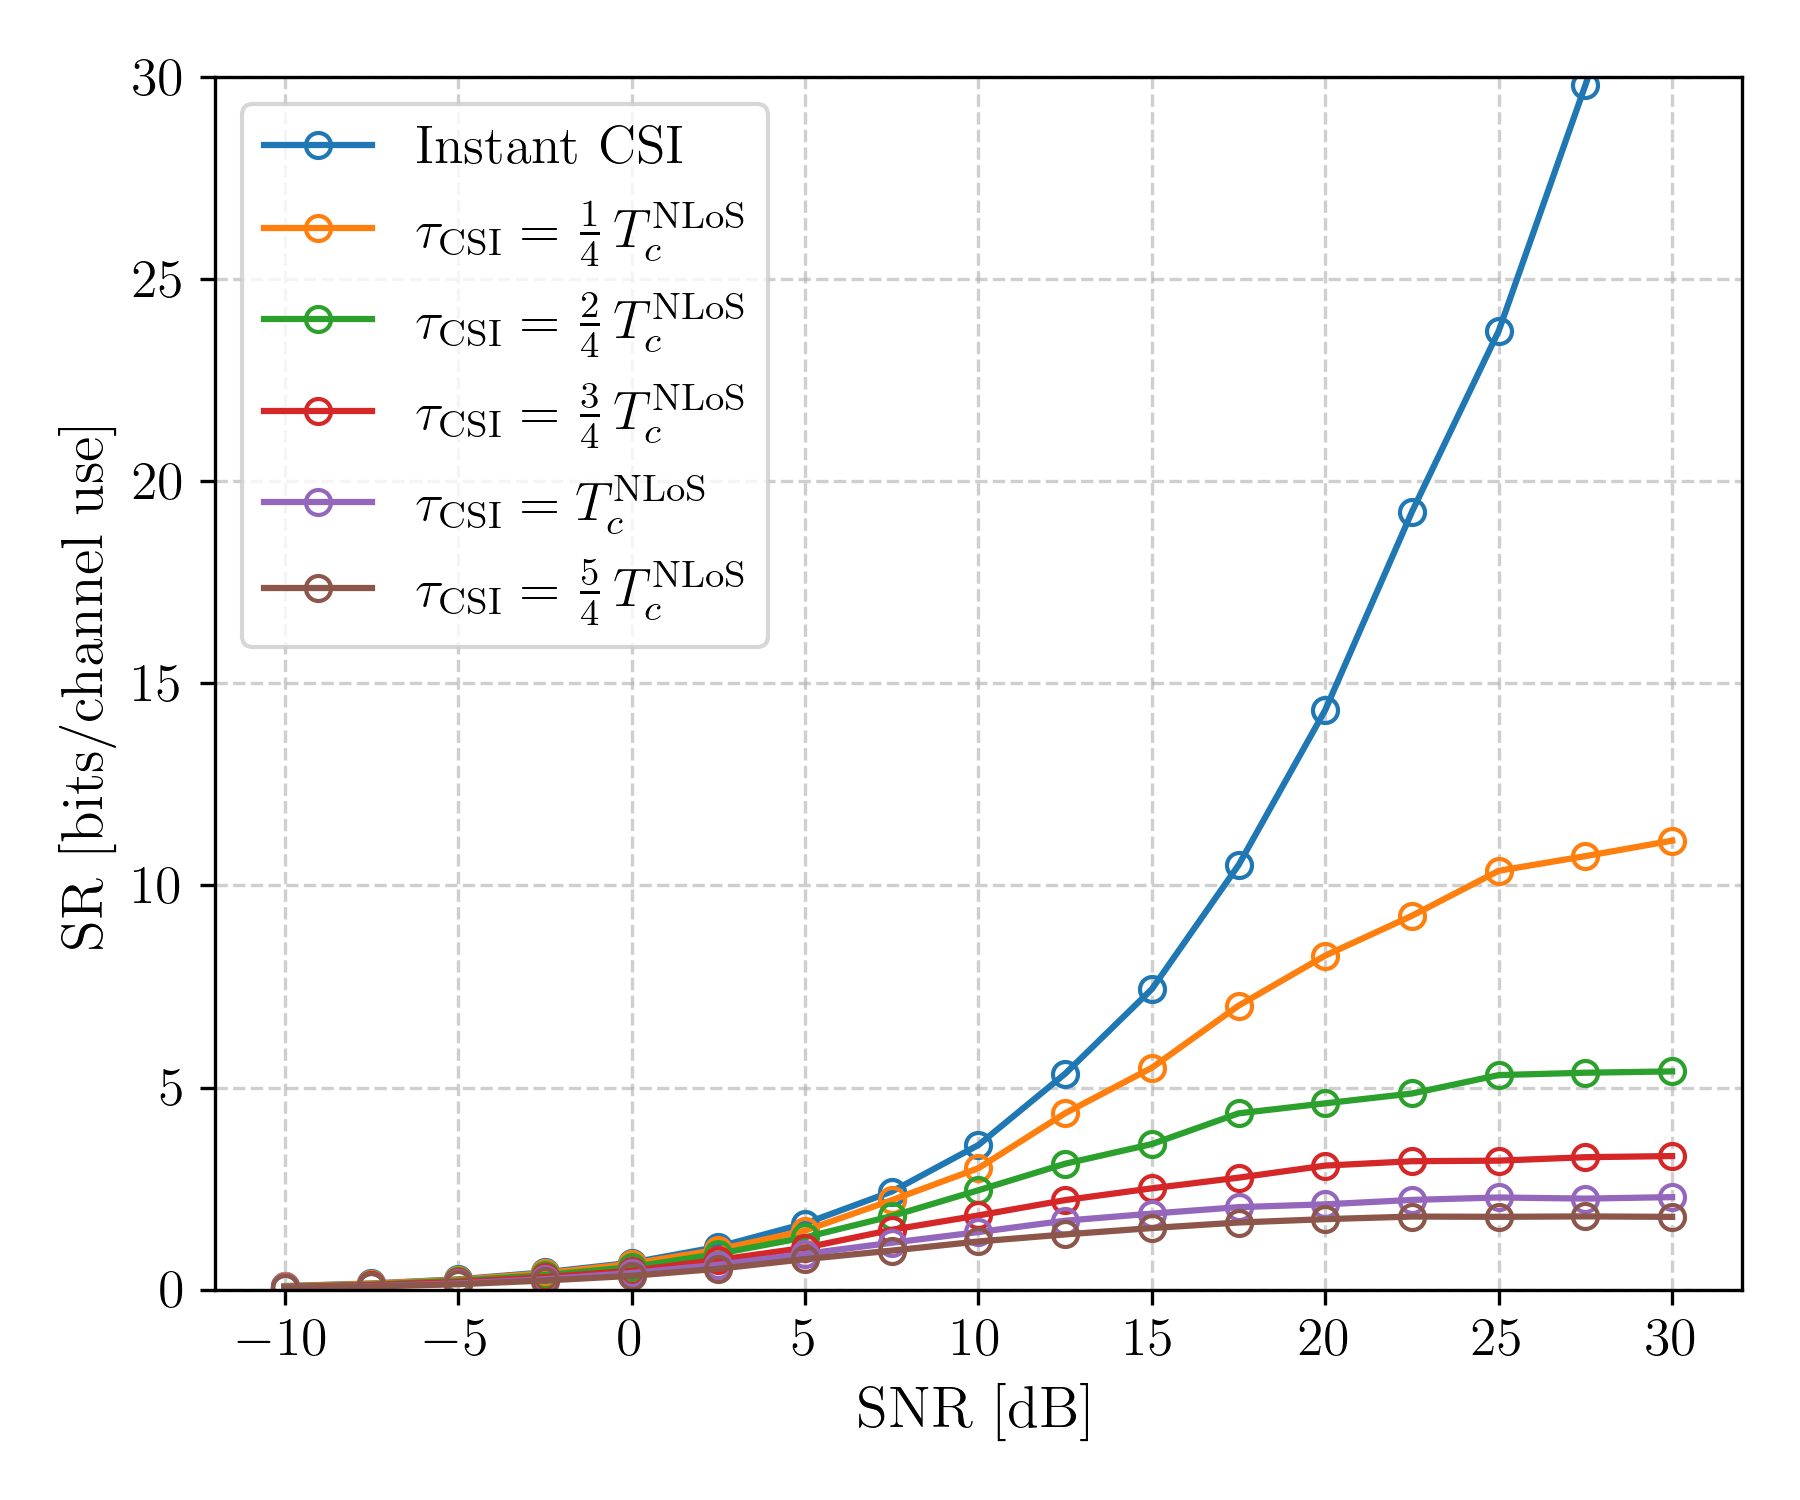
\includegraphics[width=\textwidth]{figures/satellite_communications_precoding/06_precoding_under_outdated_csi/rician_channel/impact_outdated_csi/achievable_rate_zf.png}
        \caption{\acs{ZF} Precoding}
        \label{fig:impact_outdated_csi_achievable_rate_zf}
    \end{subfigure}
    \hfill
    \begin{subfigure}{0.495\textwidth}
        \centering
        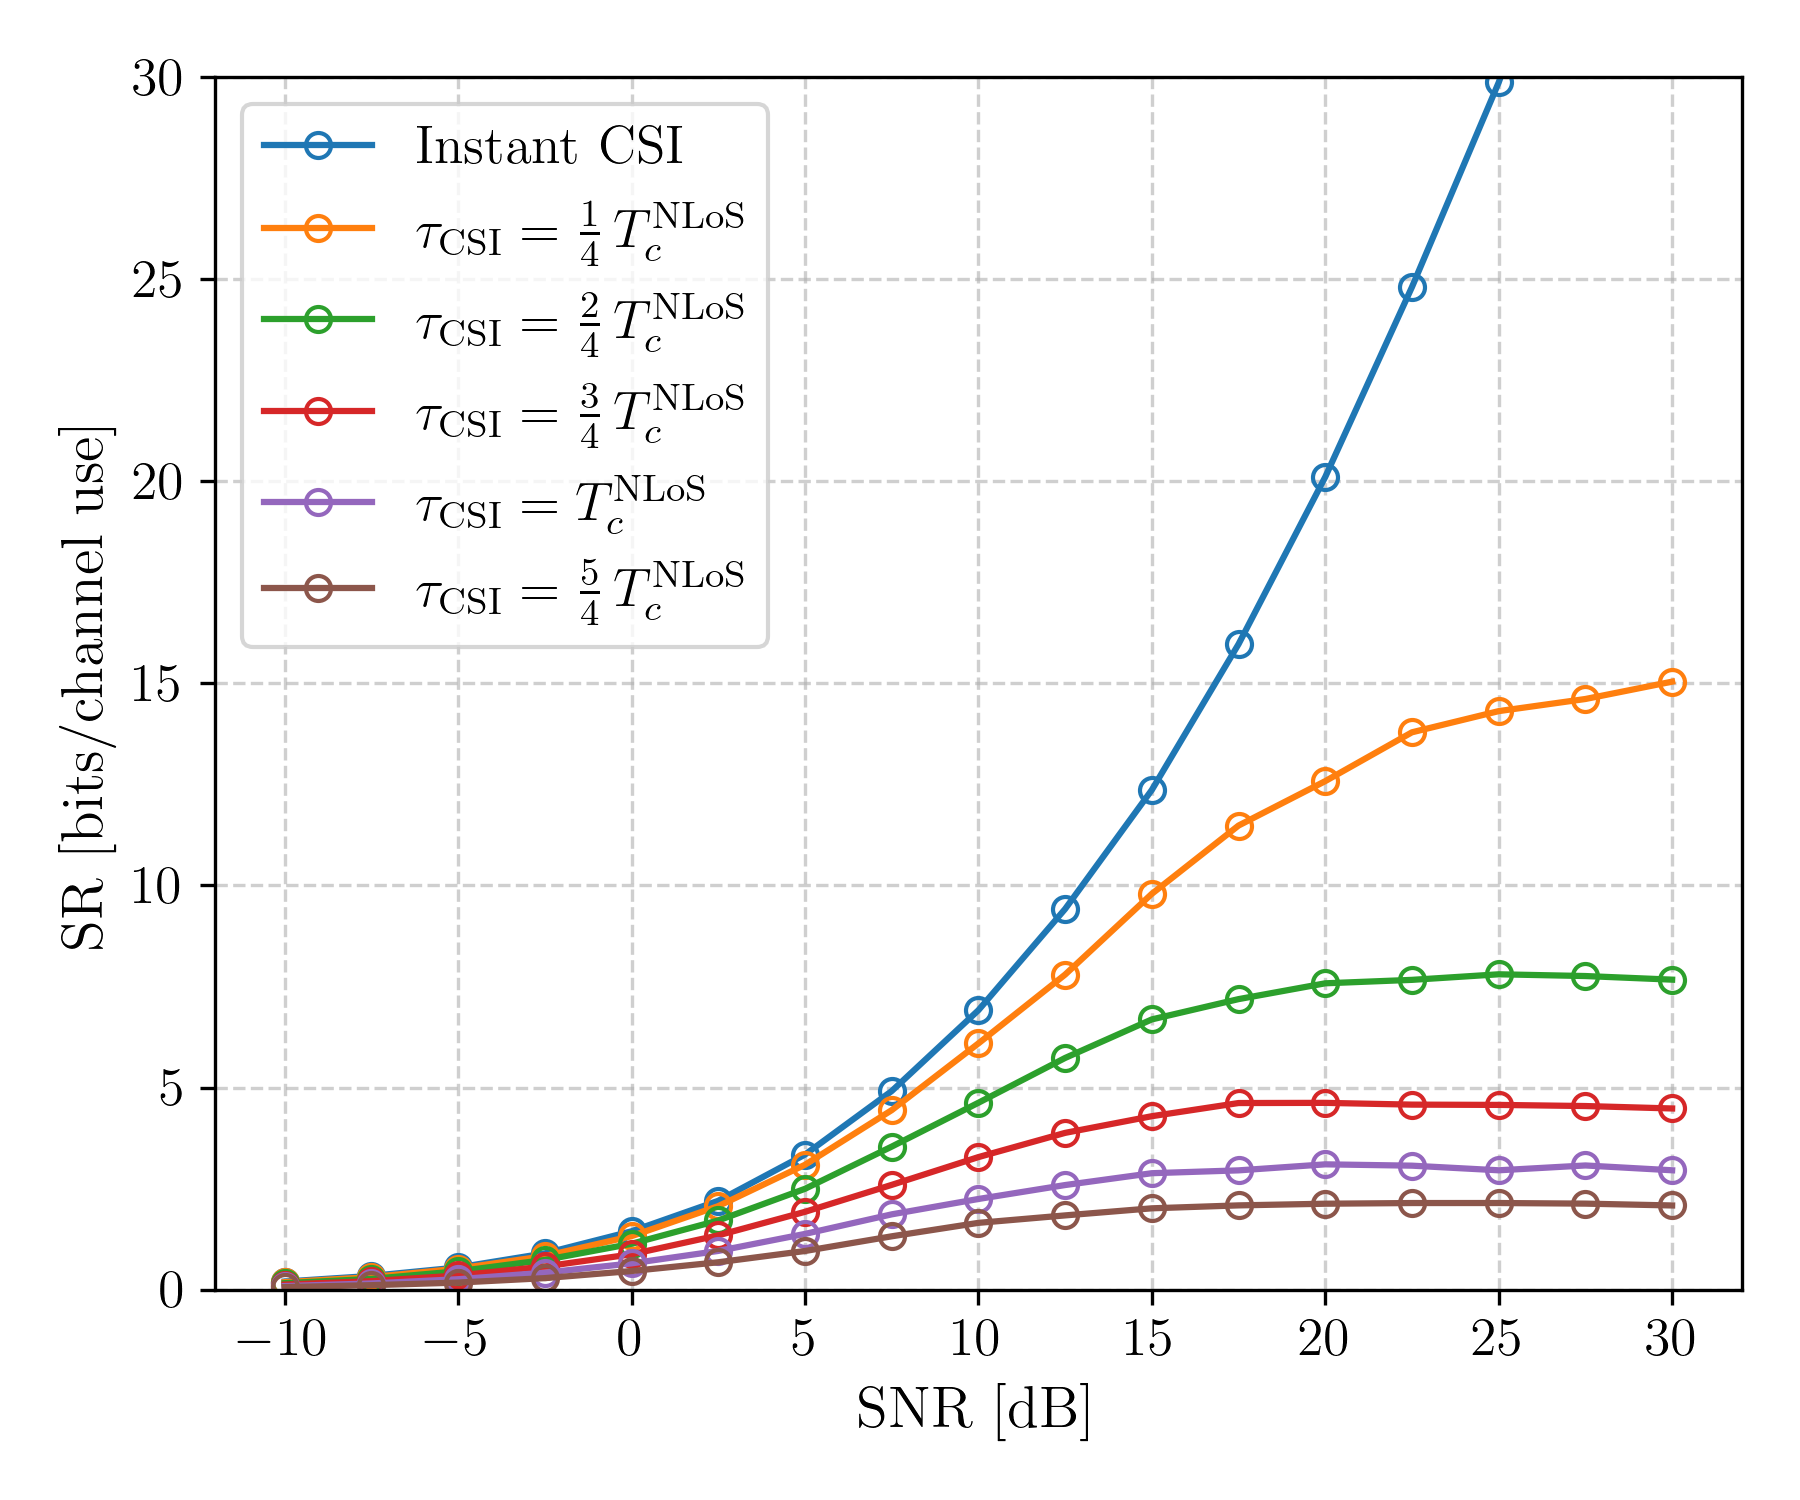
\includegraphics[width=\textwidth]{figures/satellite_communications_precoding/06_precoding_under_outdated_csi/rician_channel/impact_outdated_csi/achievable_rate_bd.png}
        \caption{\acs{BD} Precoding}
        \label{fig:impact_outdated_csi_achievable_rate_bd}
    \end{subfigure}
    \caption[Impact of outdated \acs{CSI} on the achievable sum-rate (\acs{ZF} and \acs{BD} precoding)]{
        The achievable sum-rate of a  $8 \times \{2, 2, 2, 2\} $ \acs{MU}-\acs{MIMO} system as a function of the \acs{SNR}, for \acs{ZF} and \acs{BD} precoding.
        The different curves correspond to different values of the \acs{CSI} feedback delay $\tau_{\mathrm{CSI}}$, expressed as a fraction of the coherence time $T_c$.
    }
    \label{fig:impact_outdated_csi_achievable_rate_zf_bd}
\end{figure}

% WMMSE
The \ac{WMMSE} precoder exhibits a qualitatively different behaviour.
The achievable rate reaches a maximum and decreases slightly beyond it when the precoder design relies on outdated \ac{CSI}, as is clearly visible in Figure~\ref{fig:impact_outdated_csi_achievable_rate_wmmse}.
Unlike \ac{ZF} and \ac{BD}, \ac{WMMSE} precoding adapts its solution to the operating \ac{SNR}.
At low \ac{SNR} it trades interference suppression against desired-signal power, while at high \ac{SNR} the regularization vanishes and it converges to the interference-free \ac{BD} solution.
The algorithm then increasingly concentrates power in directions that it expects to be beneficial, but which, due to the channel mismatch, actively generate inter-user interference in the actual channel.
The \ac{ZF}-type precoders do not exhibit this behaviour because they steer in the wrong direction just as aggressive for any \ac{SNR} value.

\begin{figure}[!htb]
    \centering
    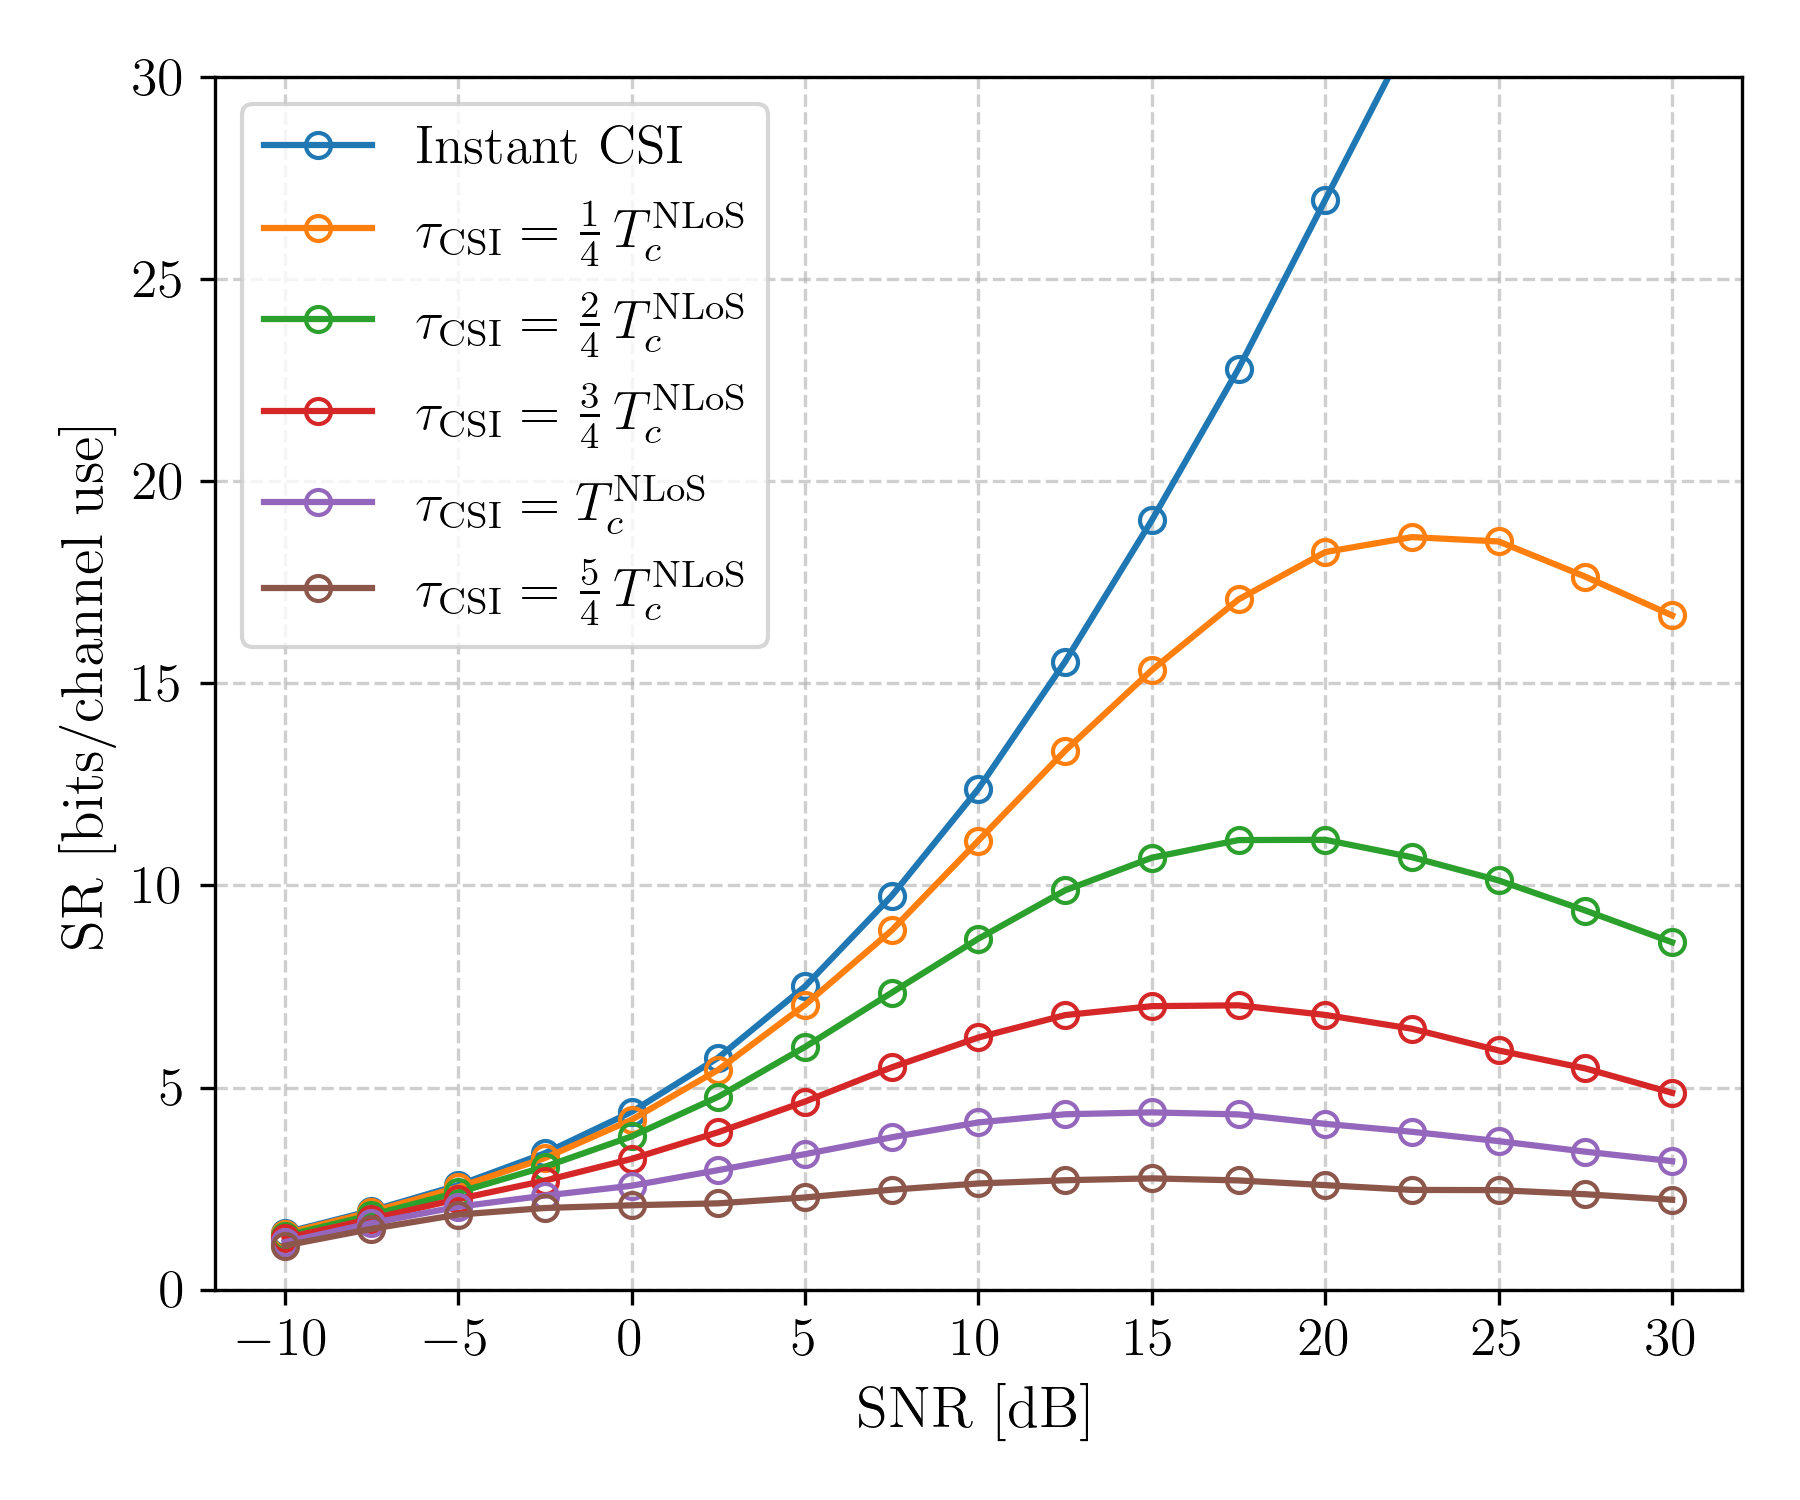
\includegraphics[width=0.65\textwidth]{figures/satellite_communications_precoding/06_precoding_under_outdated_csi/rician_channel/impact_outdated_csi/achievable_rate_wmmse.png}
    \caption[Impact of outdated \acs{CSI} on the achievable sum-rate (\acs{WMMSE} precoding)]{
        Similar figure as Fig.~\ref{fig:impact_outdated_csi_achievable_rate_zf_bd}, but for \acs{WMMSE} precoding.
    }
    \label{fig:impact_outdated_csi_achievable_rate_wmmse}
\end{figure}

% Rician vs Rayleigh
A final observation concerns the reference curve obtained with instantaneous \ac{CSI}.
Even in this idealised case, the achievable rate lies noticeably below the values obtained in Chapter~\ref{chapter:mu_mimo_precoding} under a purely Rayleigh fading channel.
This accounts for all three precoding techniques, and is a direct consequence of the \ac{LoS} contribution in a Rician channel.
Indeed, the \ac{LoS} component is rank-one, such that the largest fraction of the channel energy is concentrated along a single spatial direction.
A purely Rayleigh fading channel, by contrast, provides rich spatial diversity and a well-conditioned channel matrix, granting the precoder significantly more spatial multiplexing gain.
Therefore, the \ac{LoS} component imposes an inherent limit on the spatial degrees of freedom available, regardless of the quality of the \ac{CSI}.

% outro
Taken together, these results show that even a small feedback delay poses a threat to the achievable rate at moderate and high \ac{SNR}, and that no choice of precoder can restore the linear growth observed with instantaneous \ac{CSI} by itself.
The next section therefore turns to the design of a compensation strategy that targets the source of the mismatch, which is the temporal mismatch between $\mathbf{H}(t - \tau_{\mathrm{CSI}})$ and $\mathbf{H}(t)$, rather than its consequences.

\section{Compensation for Outdated CSI}
\label{section:outdated_csi_compensation}
% =====================================
%    Compensation for Outdated CSI
% =====================================

intro to the section

\subsection{Idea}
\label{subsection:compensation_idea}
% ----------------------------------

- explain the idea: 
use an AR model to predict the CSI for the time instant of transmission, and send the predicted version to the GW.
The GW acts as if nothing happened, all extra compensation processing happens at the UTs.
say what an AR model does, but do not go into detail, refer to Appendix~\ref{appendix:ar_models} for more info (derivation Yule-Walker equations, ...)

- explain the assumptions
the UTs have access to the statisctic of the channel
further, we will assume that the rate of pilot messages is not constraint but free to choose.


\subsection{AR parameter optimization}
\label{subsection:compensation_ar_model_parameter_optimization}
% -------------------------------------------------------------

- explain the free parameters of the AR model
the pilot message rate. this corresponds to the frequency of the taps of the AR model.
the context window length. this determines the size of the memory at the UT, and how much in the past we look te predict the future channel impulse response.

- shortly go through the optimization process.
instead of a full grid search over the window length, the order of the ar-model and the delay of the CSI feedback (~ propagation delay), we first choose a fixed number of taps, and then fix the number of tabs to that number. Then, we choose the best window length.


we start with a window length of 1.5 Tc. This is a reasonable choice. We do not expect a lot of useful information to be lost with this length.
plot the achievable rate with compensation as a function of the number of tabs (with a fixed window length of 1.5).
the number of tabs the model uses is directly correlated to the pilot message rate. (number of tabs equals pilot message rate times the context window length)
hypothesis: the higher the pilot range, the better the prediction quality (more information accessible)
the hypothesis is correct. 
Figure~\ref{fig:parameter_pilot_rate} shows that using to few taps can drastically decrease the quality of the prediction and therefore the achievable sum-rate of the system when using the compensation technique compared to more taps.
The use of the 6 pilot messages per coherence times seems ideal. There is even a slight decrease in performance when using more taps.

\begin{figure}[!htb]
    \centering
    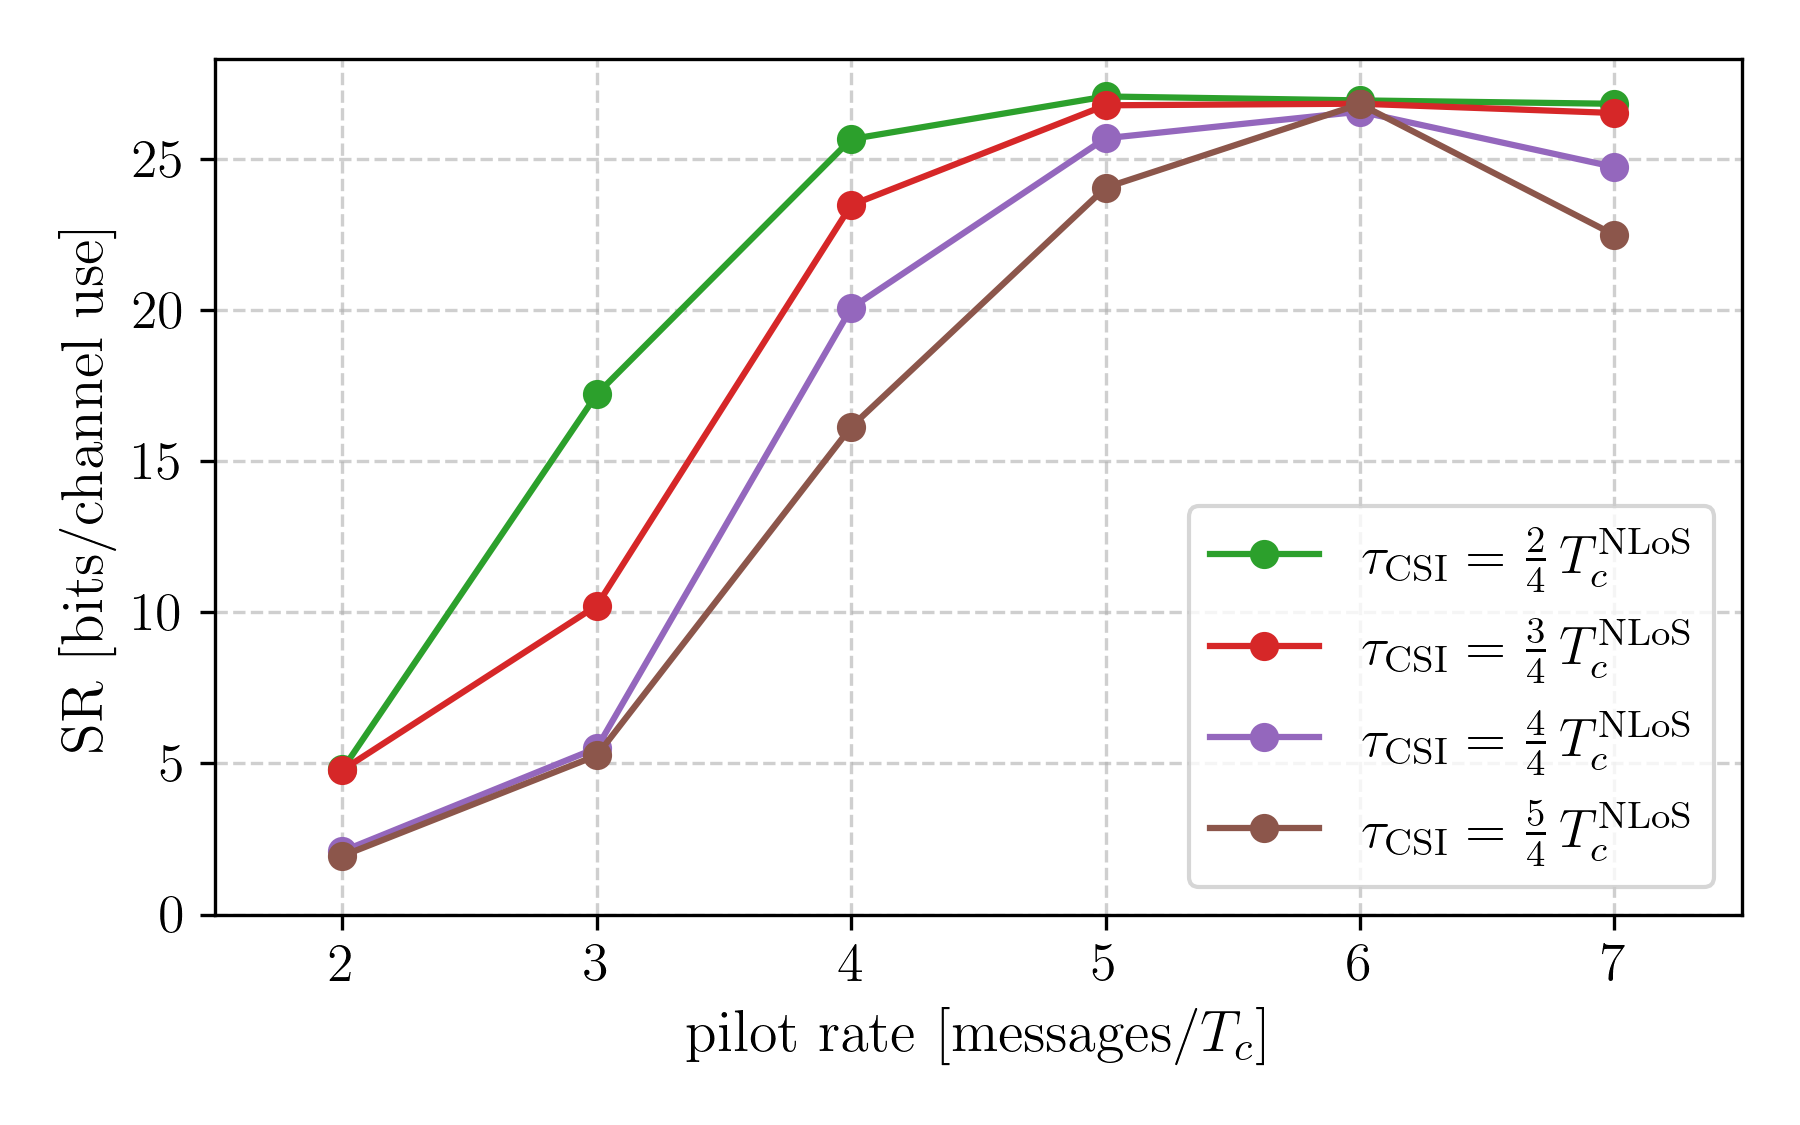
\includegraphics[width=0.65\textwidth]{figures/satellite_communications_precoding/06_precoding_under_outdated_csi/rician_channel/ar_model_parameter_choice/pilot_rate_wmmse.png}
    \caption[Impact of the pilot message rate on the achievable sum-rate]{
        The impact of the pilot message rate on the achievable sum-rate of a $8 \times \{2, 2, 2, 2\}$ system using \acs{WMMSE} precoding at an operating point with an \acs{SNR} of $20~\mathbf{dB}$. 
        The different curves represent different \acs{CSI} feedback delays.
        The context window length is fixed to $1.5 \, T_c$.
    }
    \label{fig:parameter_pilot_rate}
\end{figure}

next, we optimize the context window length, which corresponds to the memory size of the \ac{AR}-model.
hypothesis: the longer the context window, the better the prediction and thus the system performance. A longer window will not harm the performance, since it only adds extra (useless) information.
the hypothesis gets acknowledged by figure~\ref{fig:parameter_context_window_length_wmmse}.
The figure shows that a too short context window length can drastically decrease the achievable sum-rate.
Once the context window exceeds 1 Tc, no additional increase in achievable sum-rate is observed for the plotted values of CSI feedback delay.
We choose the context window length equal to 1 Tc

\begin{figure}[!htb]
    \centering
    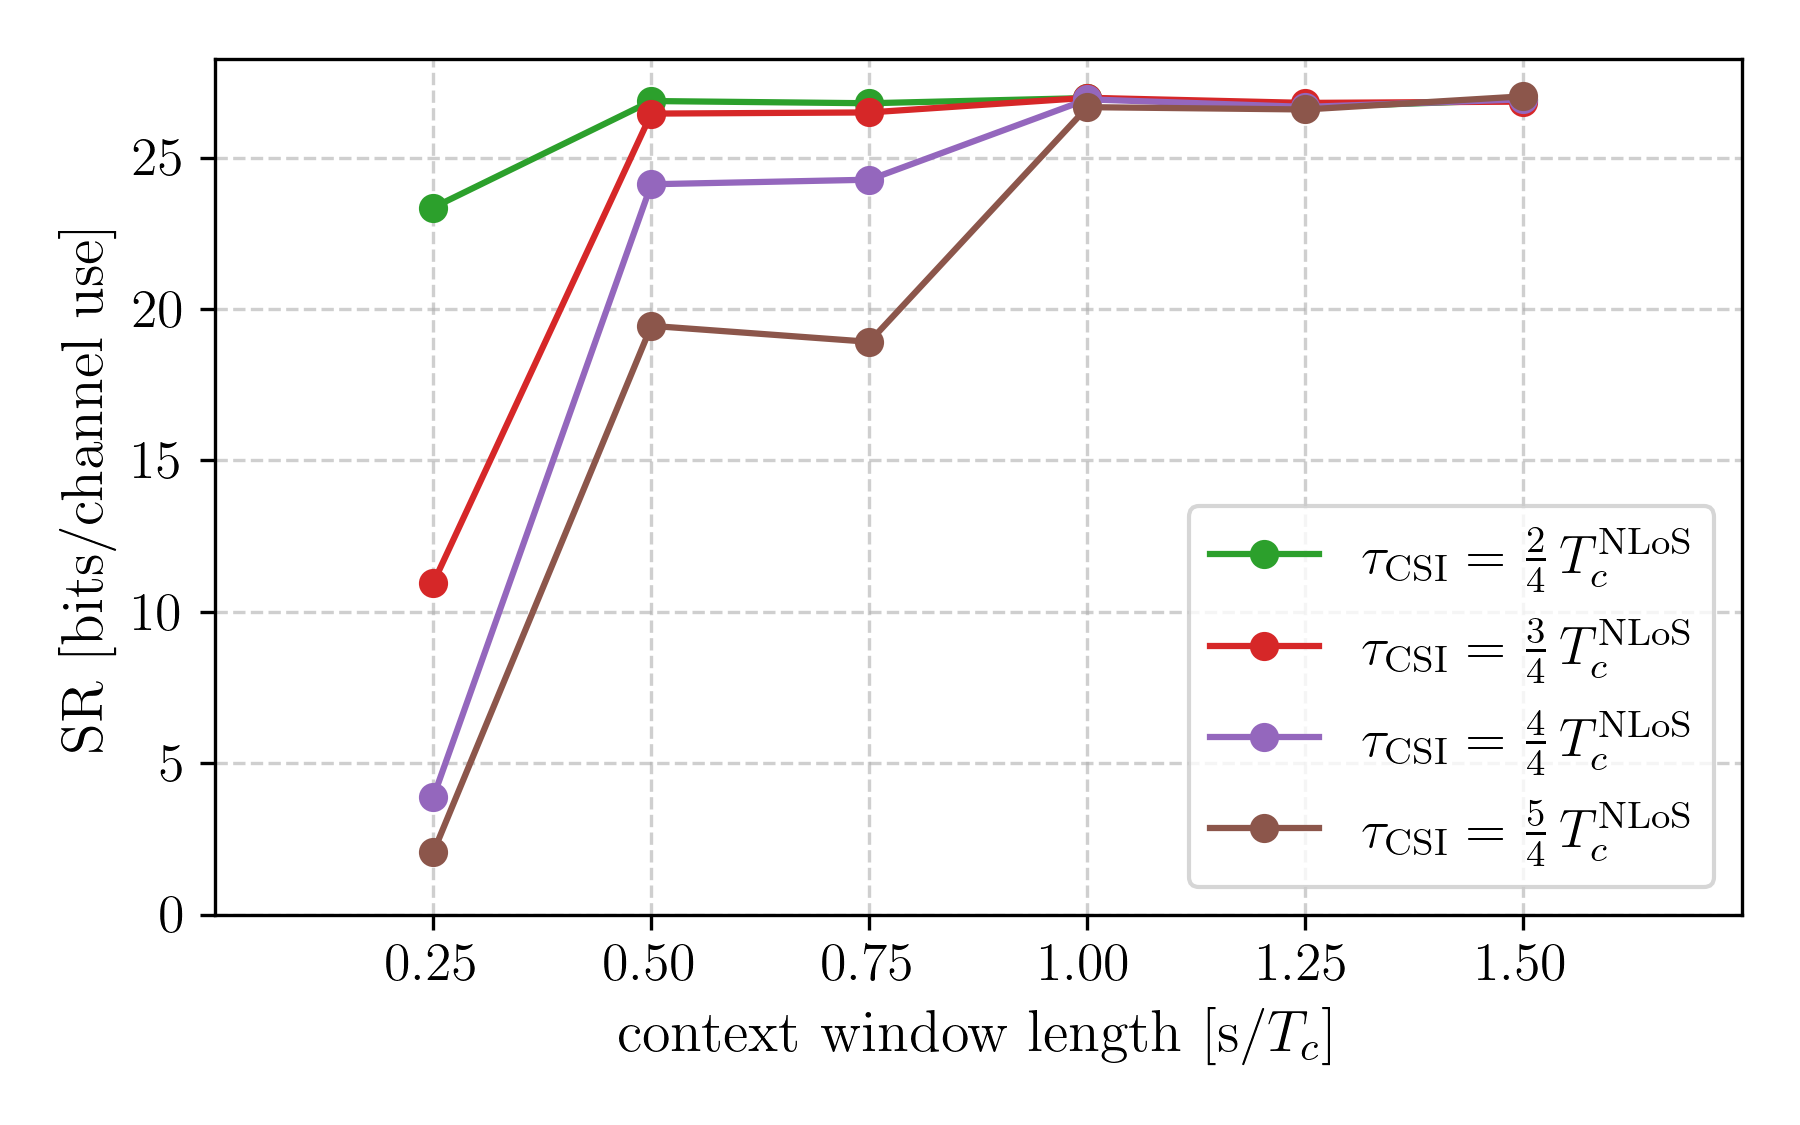
\includegraphics[width=0.65\textwidth]{figures/satellite_communications_precoding/06_precoding_under_outdated_csi/rician_channel/ar_model_parameter_choice/context_window_length_wmmse.png}
    \caption[Impact of context window length of the \acs{AR}-model on the achievable sum-rate]{
        The impact of context window length of the \acs{AR}-model on the achievable sum-rate of a $8 \times \{2, 2, 2, 2\}$ system using \acs{WMMSE} precoding sing \acs{WMMSE} precoding at an operating point with an \acs{SNR} of $20~\mathbf{dB}$. 
        The different curves represent different \acs{CSI} feedback delays.
        The number of taps id fixed to $6$.
    }
    \label{fig:parameter_context_window_length_wmmse}
\end{figure}



\subsection{Simulation Results}
\label{subsection:compensation_simulation_results}
% ------------------------------------------------


\begin{figure}[!htb]
    \centering
    \begin{subfigure}{0.495\textwidth}
        \centering
        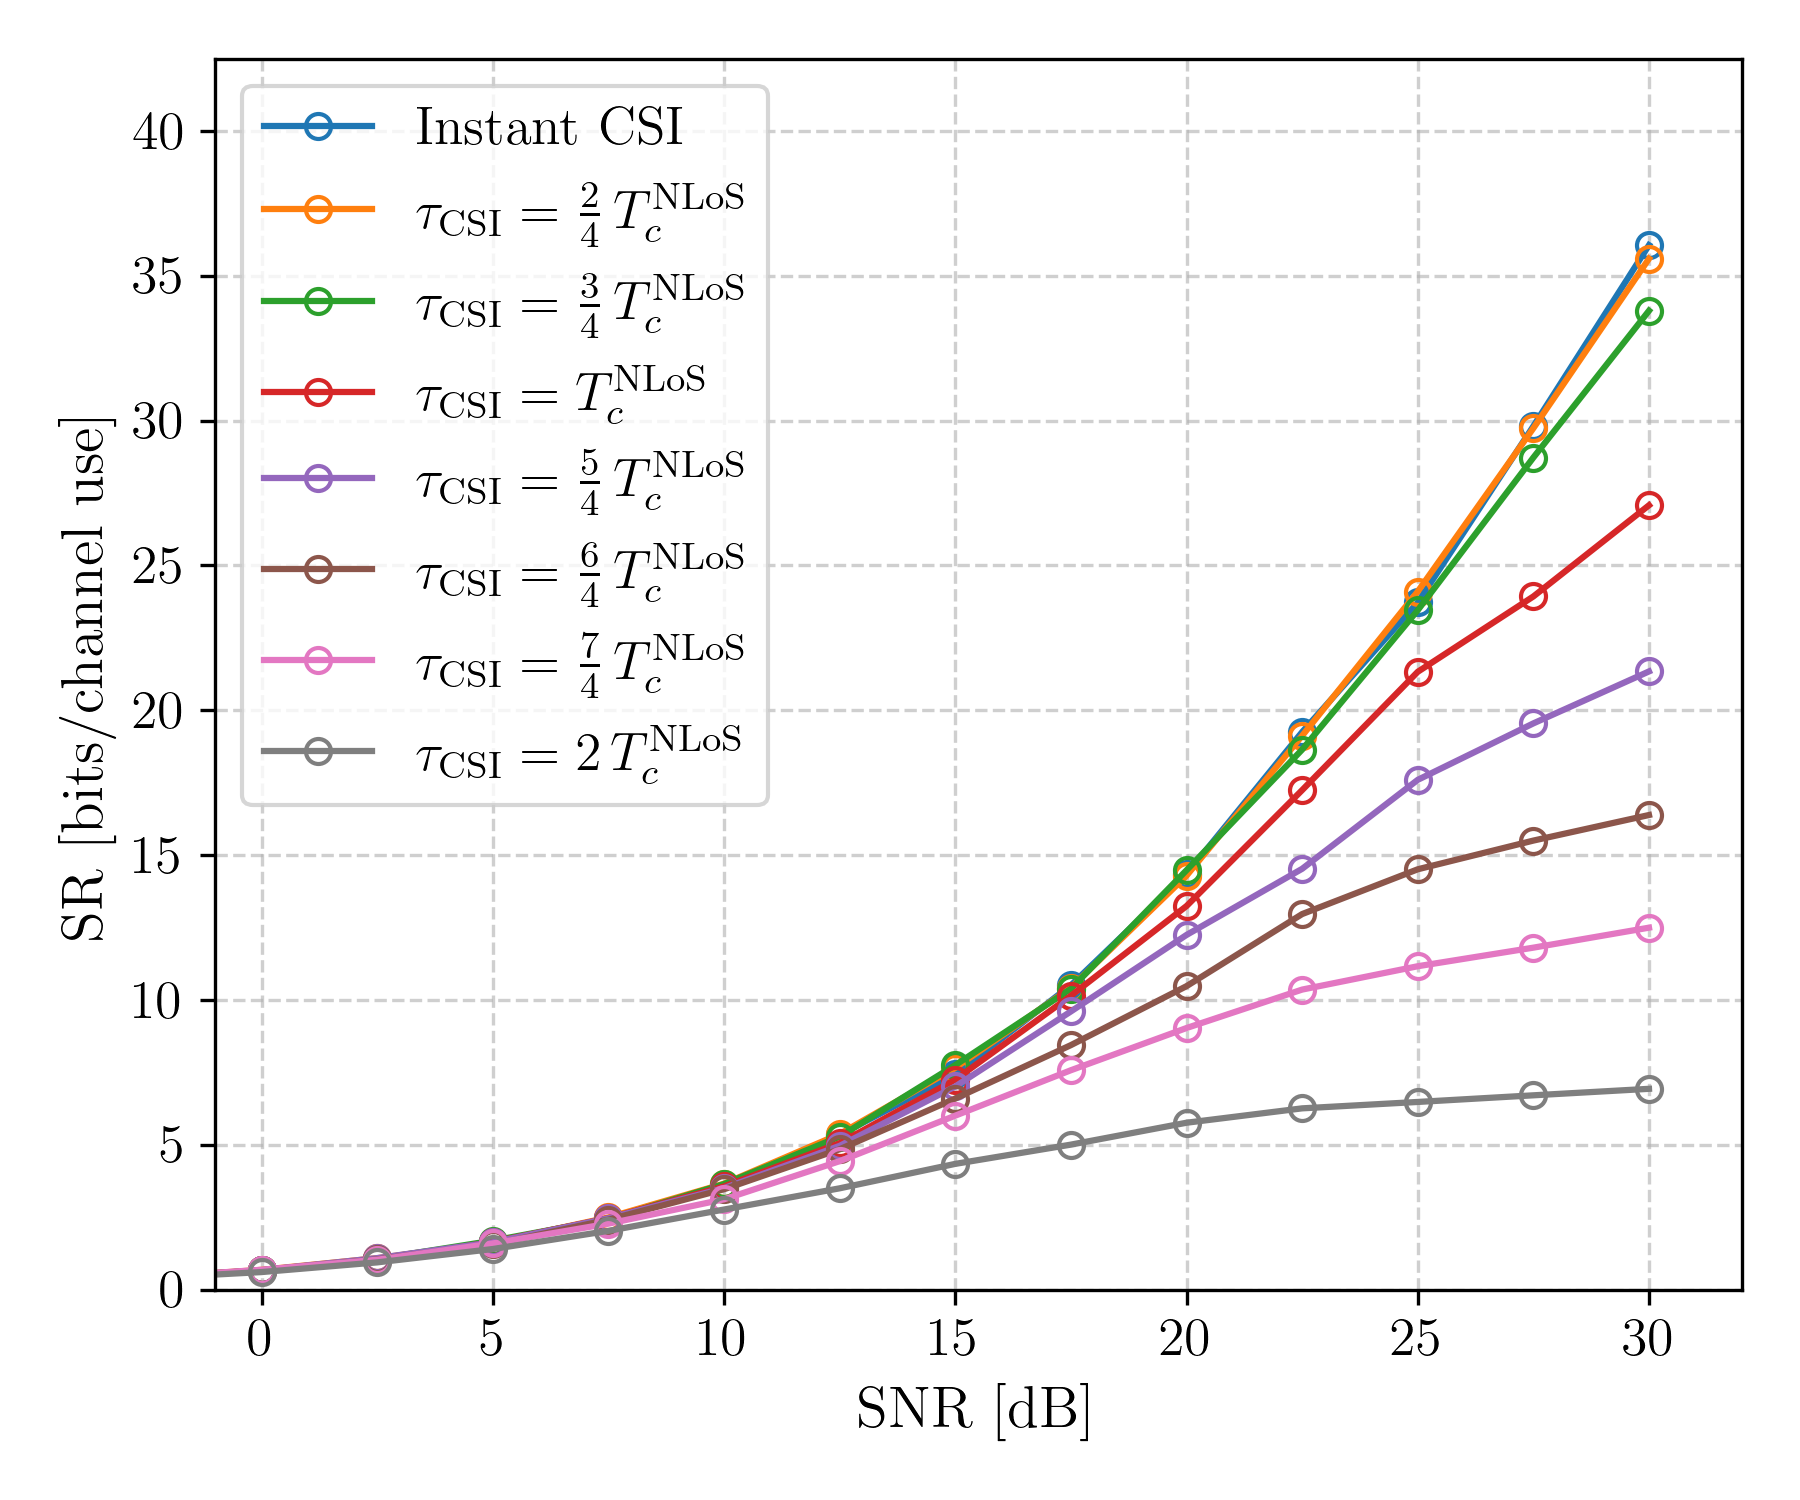
\includegraphics[width=\textwidth]{figures/satellite_communications_precoding/06_precoding_under_outdated_csi/rician_channel/impact_compensation/achievable_rate_zf.png}
        \caption{\acs{ZF} Precoding}
        \label{fig:impact_compensation_achievable_rate_zf}
    \end{subfigure}
    \hfill
    \begin{subfigure}{0.495\textwidth}
        \centering
        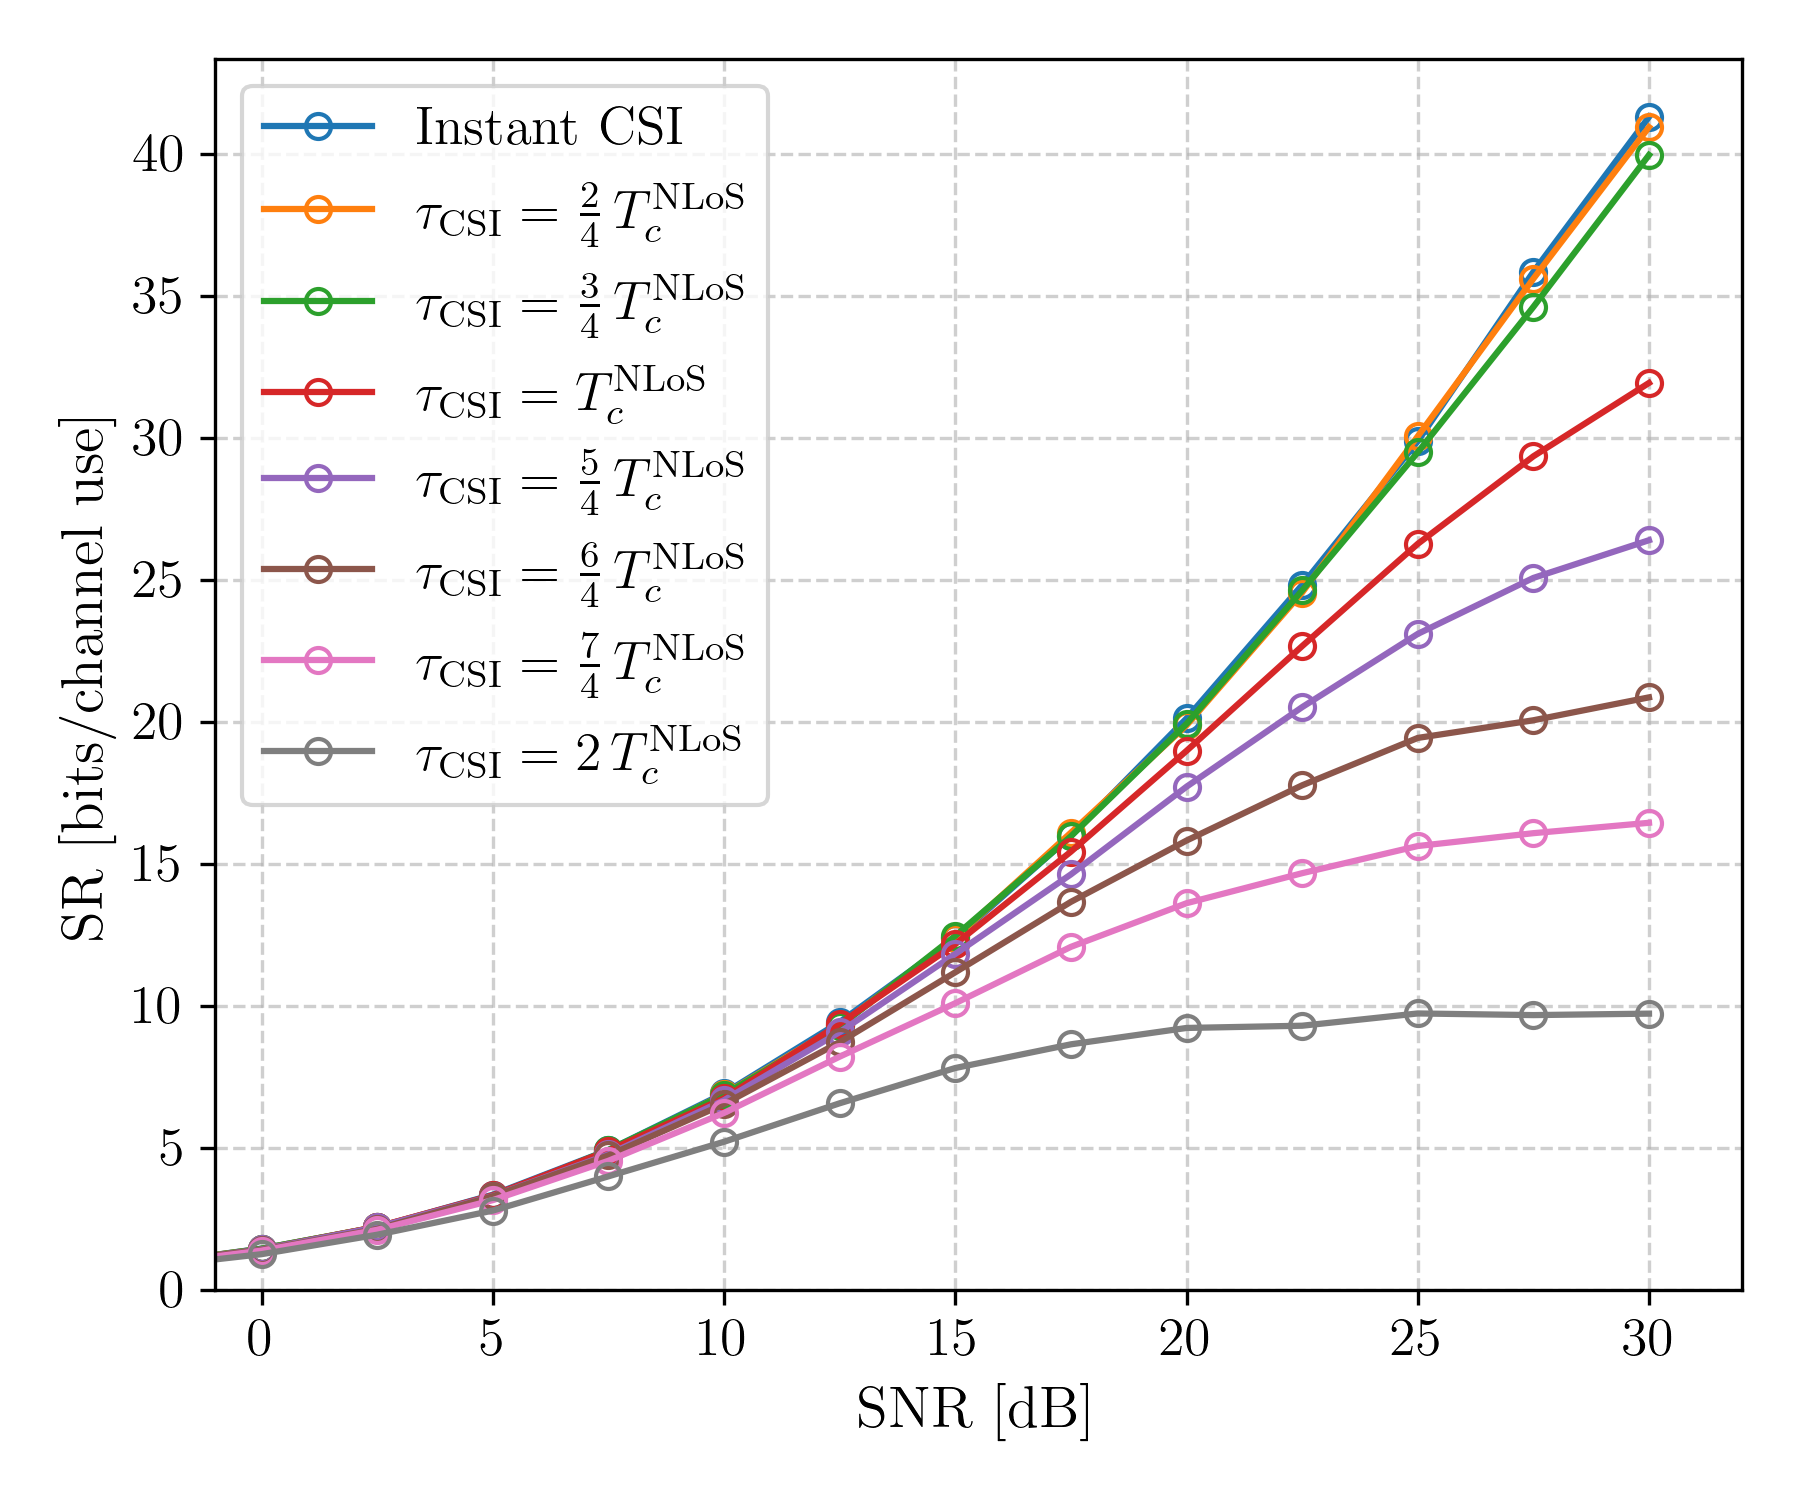
\includegraphics[width=\textwidth]{figures/satellite_communications_precoding/06_precoding_under_outdated_csi/rician_channel/impact_compensation/achievable_rate_bd.png}
        \caption{\acs{BD} Precoding}
        \label{fig:impact_compensation_achievable_rate_bd}
    \end{subfigure}
    \caption[Impact of the proposed compensation method for outdated \acs{CSI} on the achievable rate (\acs{ZF} and \acs{BD} precoding)]{
        TO DO
    }
    \label{fig:impact_compensation_achievable_rate_zf_bd}
\end{figure}
 
\begin{figure}[htb!]
    \centering

    \makebox[\textwidth][c]{%
        \begin{minipage}{1.2\textwidth}
            \centering

            % First row
            \begin{subfigure}{0.245\textwidth}
                \centering
                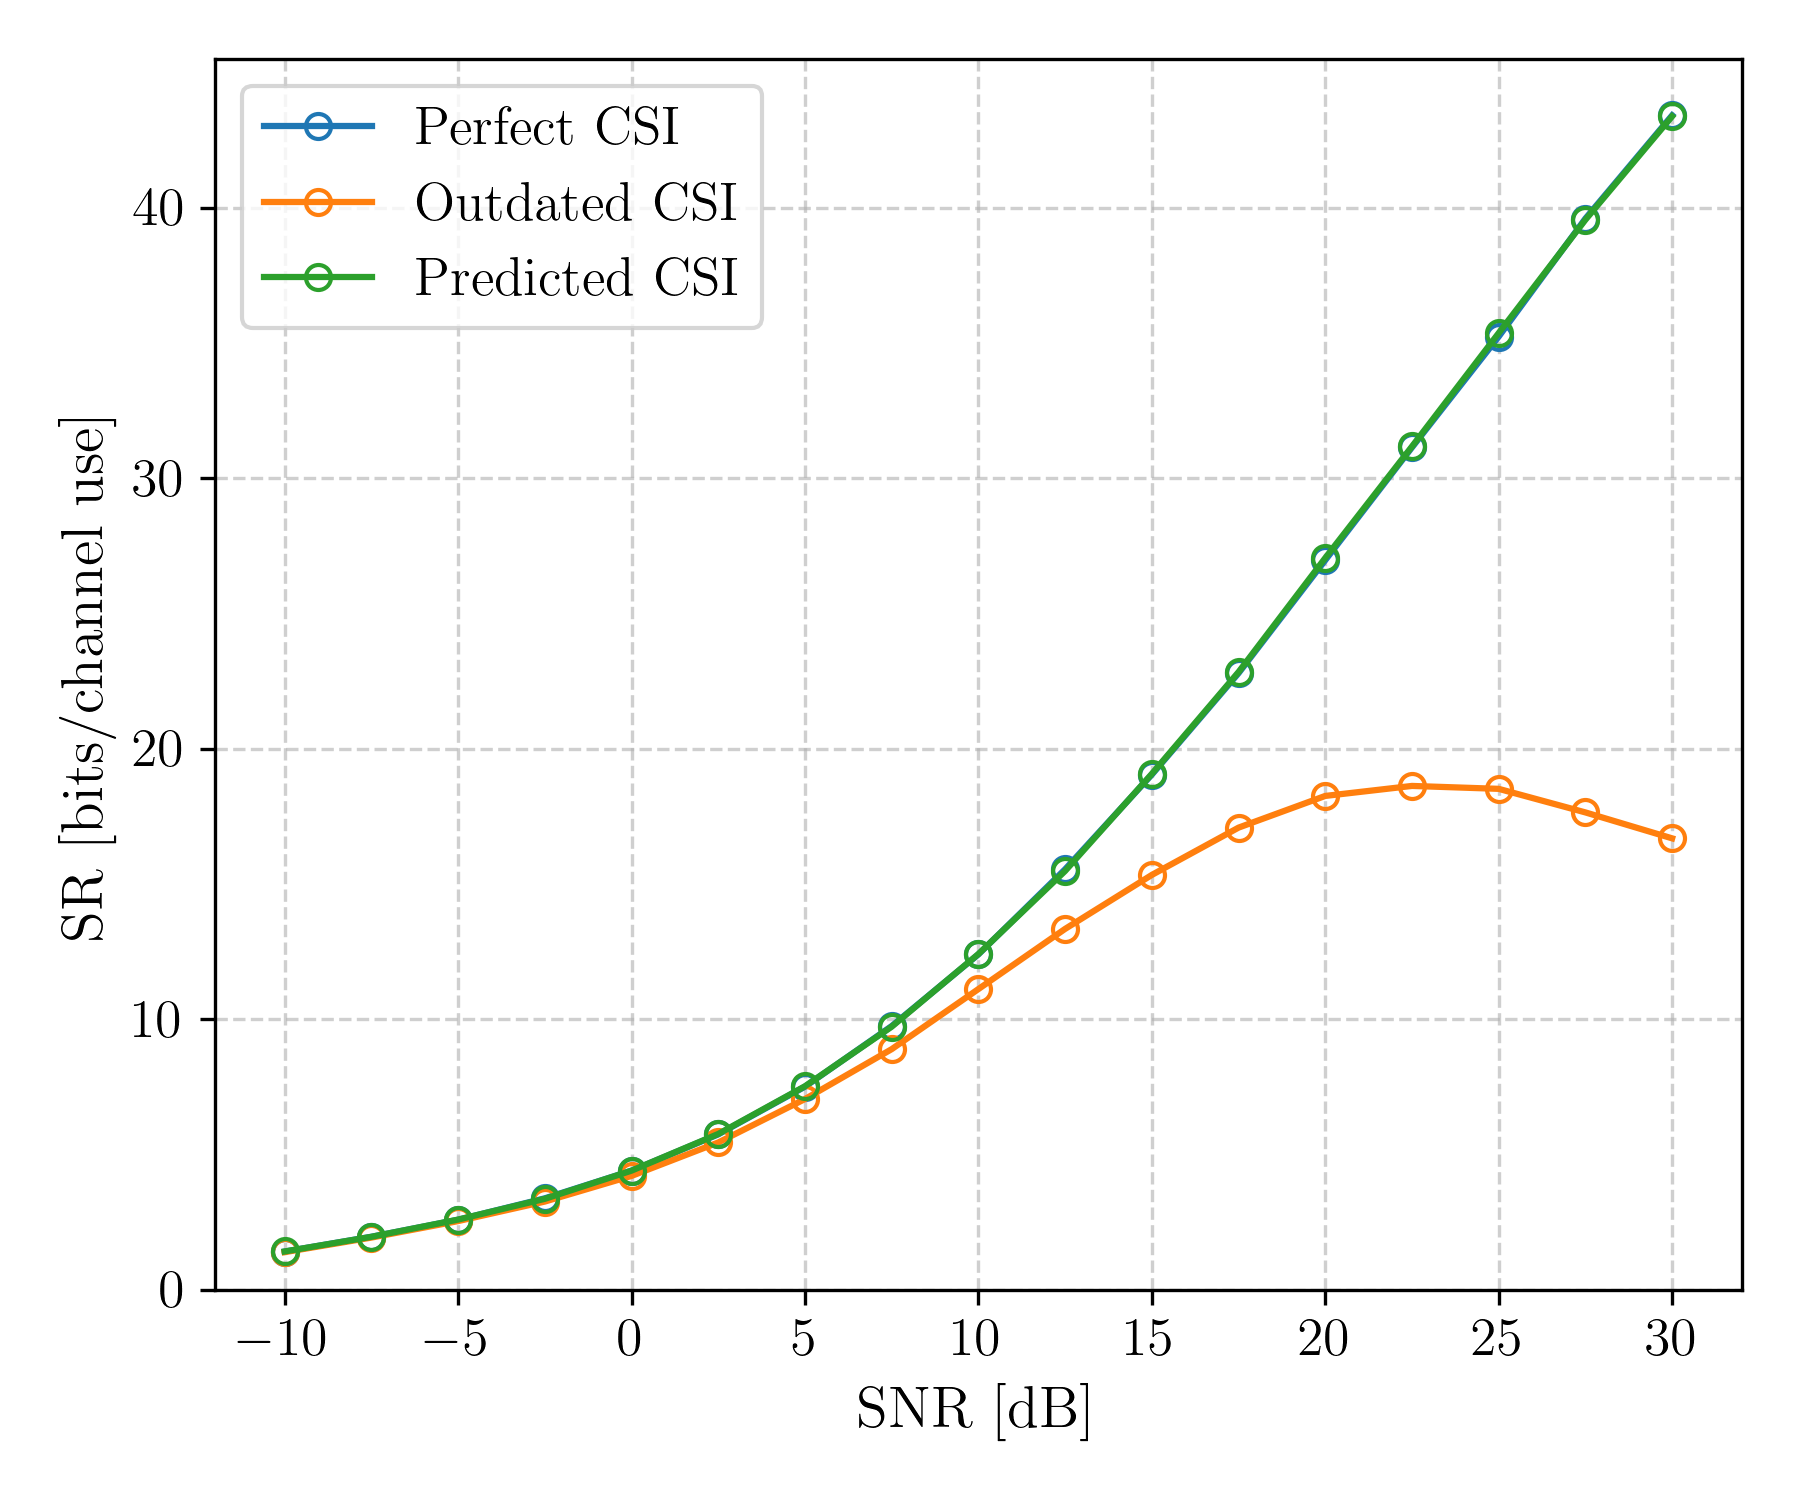
\includegraphics[width=\textwidth]{figures/satellite_communications_precoding/06_precoding_under_outdated_csi/rician_channel/impact_compensation/comparisons/wmmse/1on4.png}
                \caption{$\tau_{\mathrm{CSI}} = \frac{1}{4} T_c$}
            \end{subfigure}
            \hfill
            \begin{subfigure}{0.245\textwidth}
                \centering
                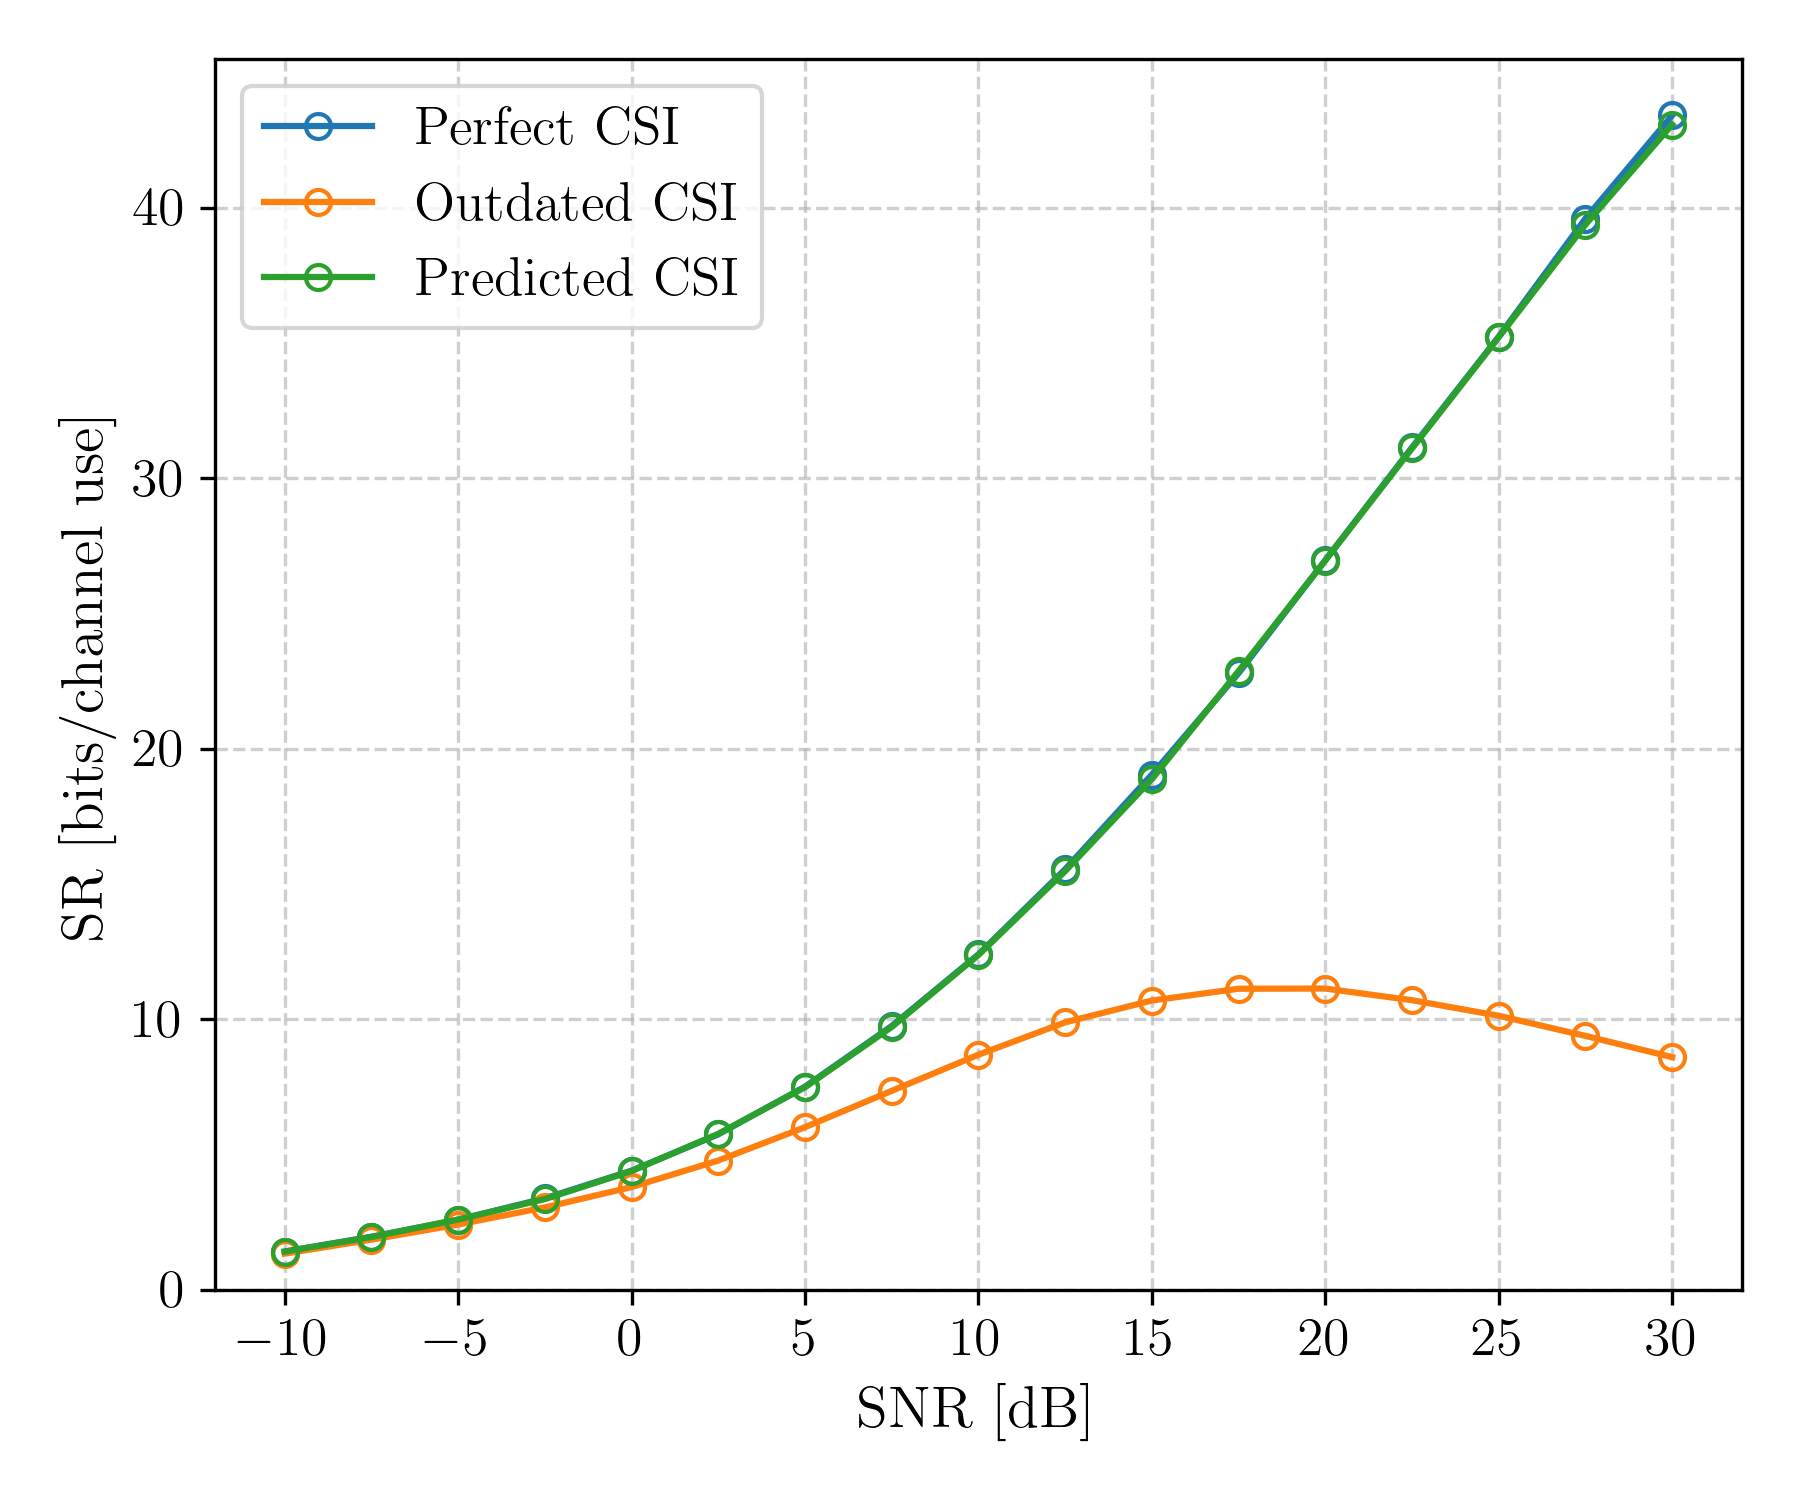
\includegraphics[width=\textwidth]{figures/satellite_communications_precoding/06_precoding_under_outdated_csi/rician_channel/impact_compensation/comparisons/wmmse/2on4.png}
                \caption{$\tau_{\mathrm{CSI}} = \frac{2}{4} T_c$}
            \end{subfigure}
            \hfill
            \begin{subfigure}{0.245\textwidth}
                \centering
                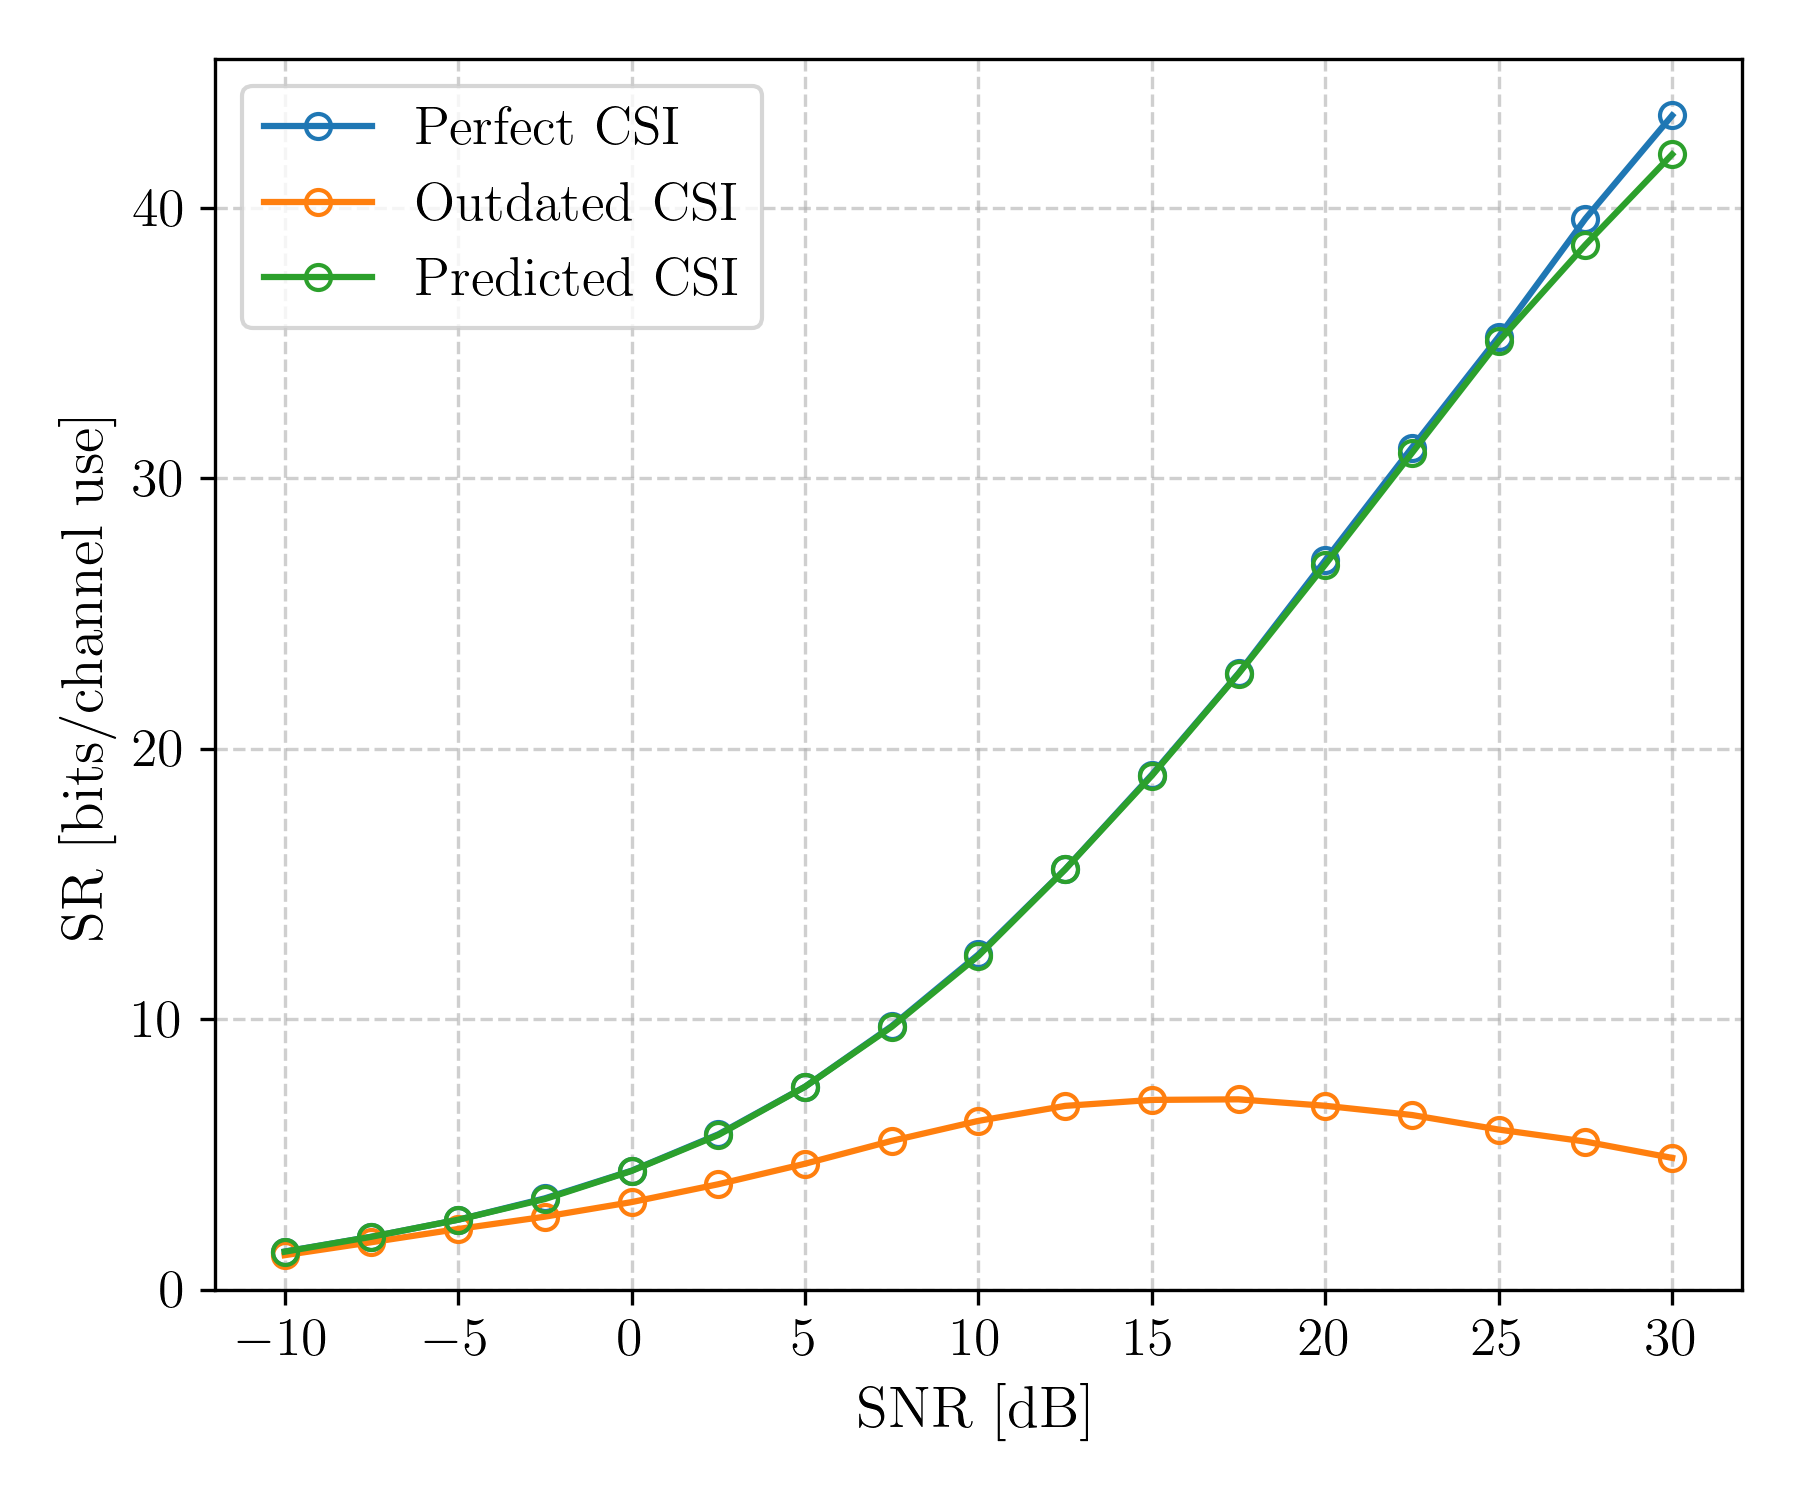
\includegraphics[width=\textwidth]{figures/satellite_communications_precoding/06_precoding_under_outdated_csi/rician_channel/impact_compensation/comparisons/wmmse/3on4.png}
                \caption{$\tau_{\mathrm{CSI}} = \frac{3}{4} T_c$}
            \end{subfigure}
            \hfill
            \begin{subfigure}{0.245\textwidth}
                \centering
                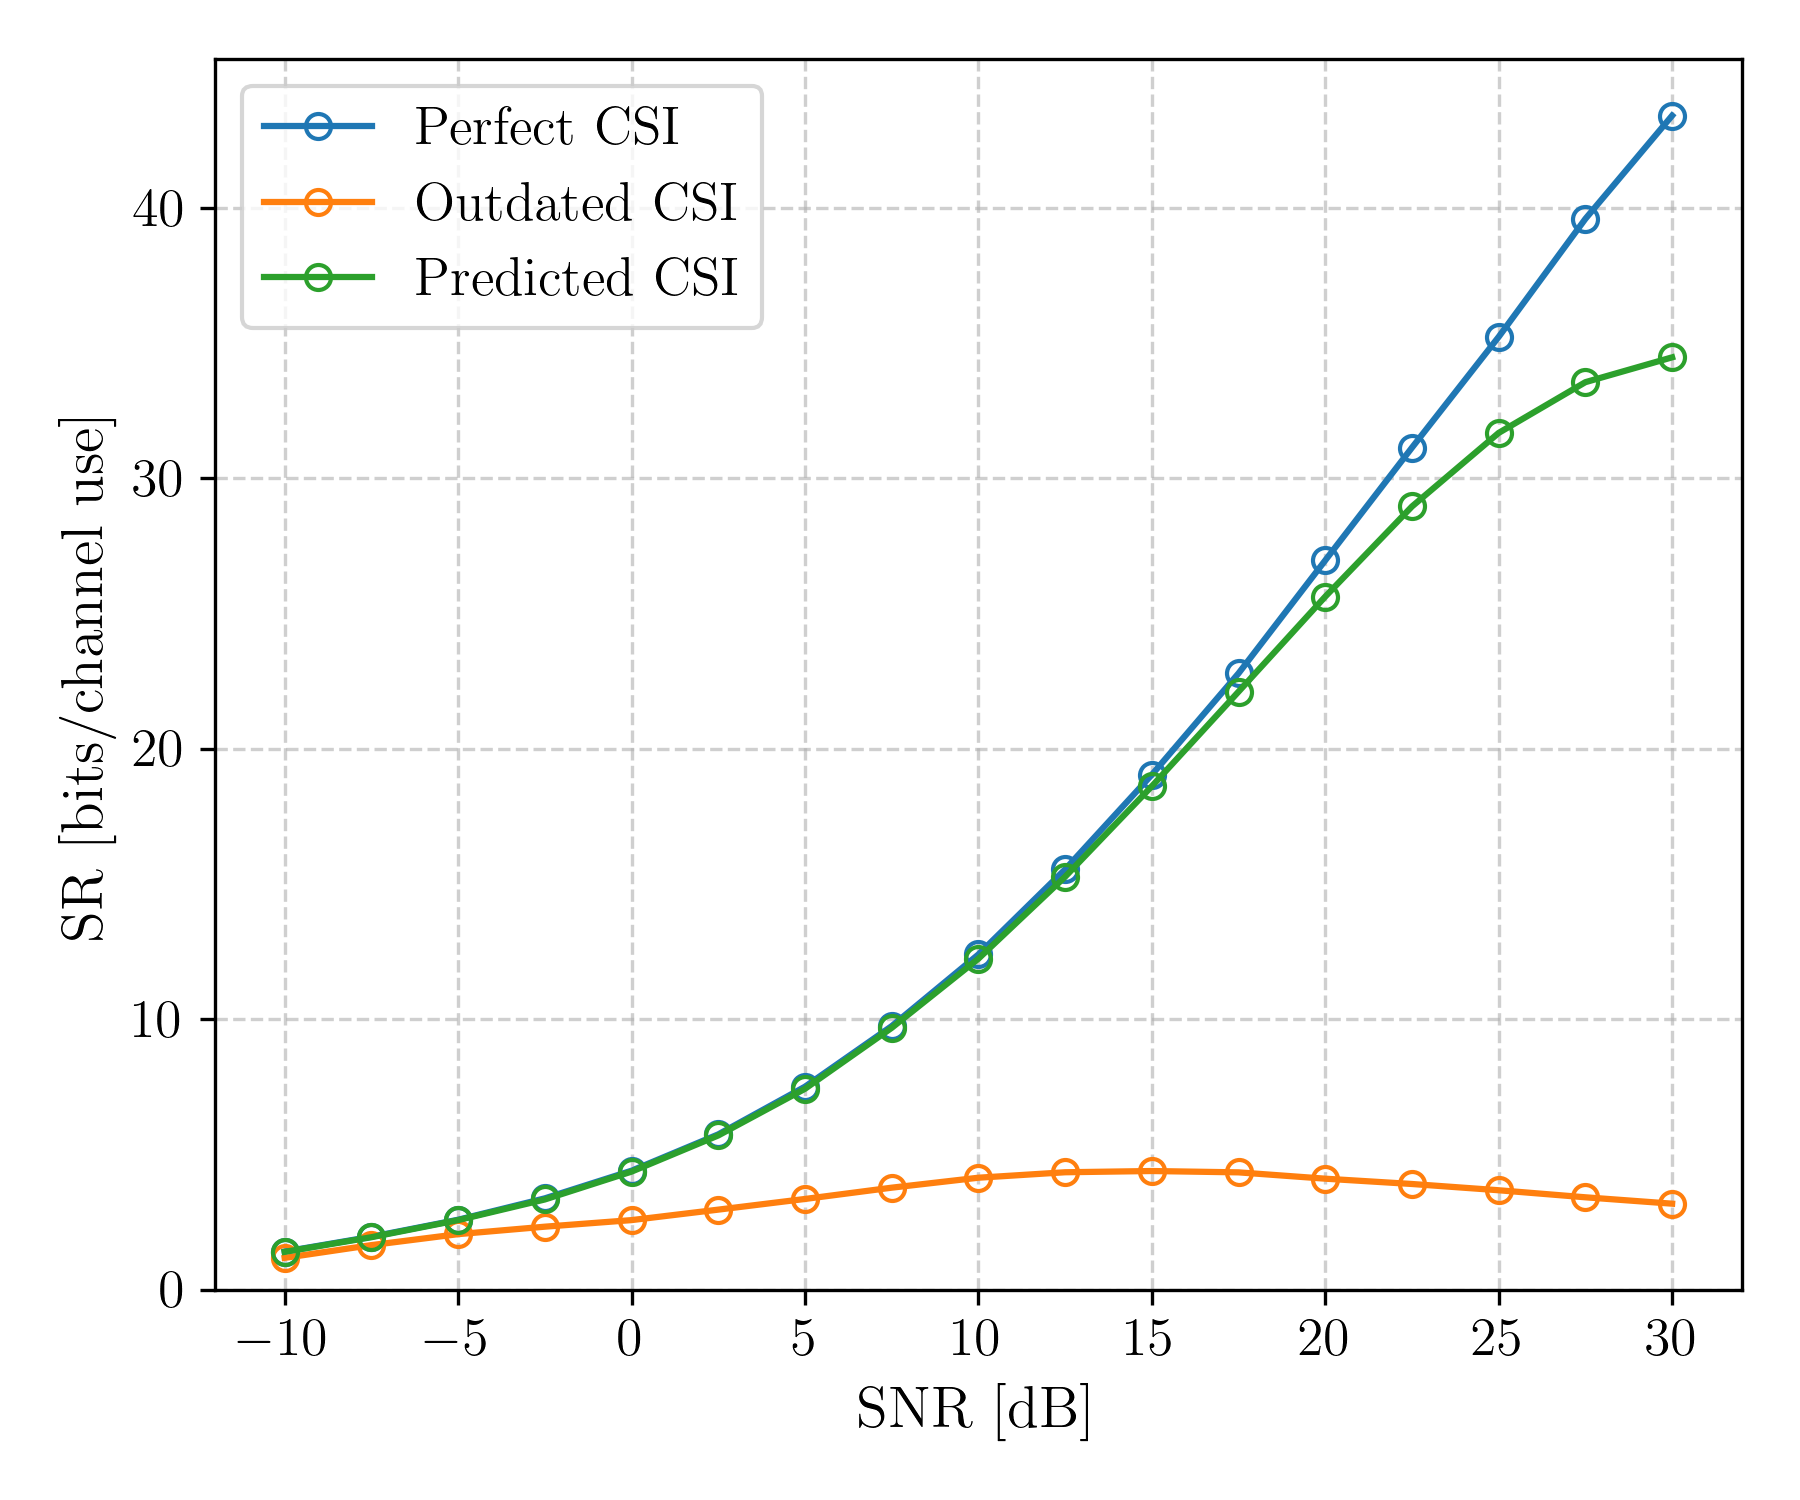
\includegraphics[width=\textwidth]{figures/satellite_communications_precoding/06_precoding_under_outdated_csi/rician_channel/impact_compensation/comparisons/wmmse/4on4.png}
                \caption{$\tau_{\mathrm{CSI}} = \frac{4}{4} T_c$}
            \end{subfigure}

            \vspace{0.5cm}

            % Second row
            \begin{subfigure}{0.245\textwidth}
                \centering
                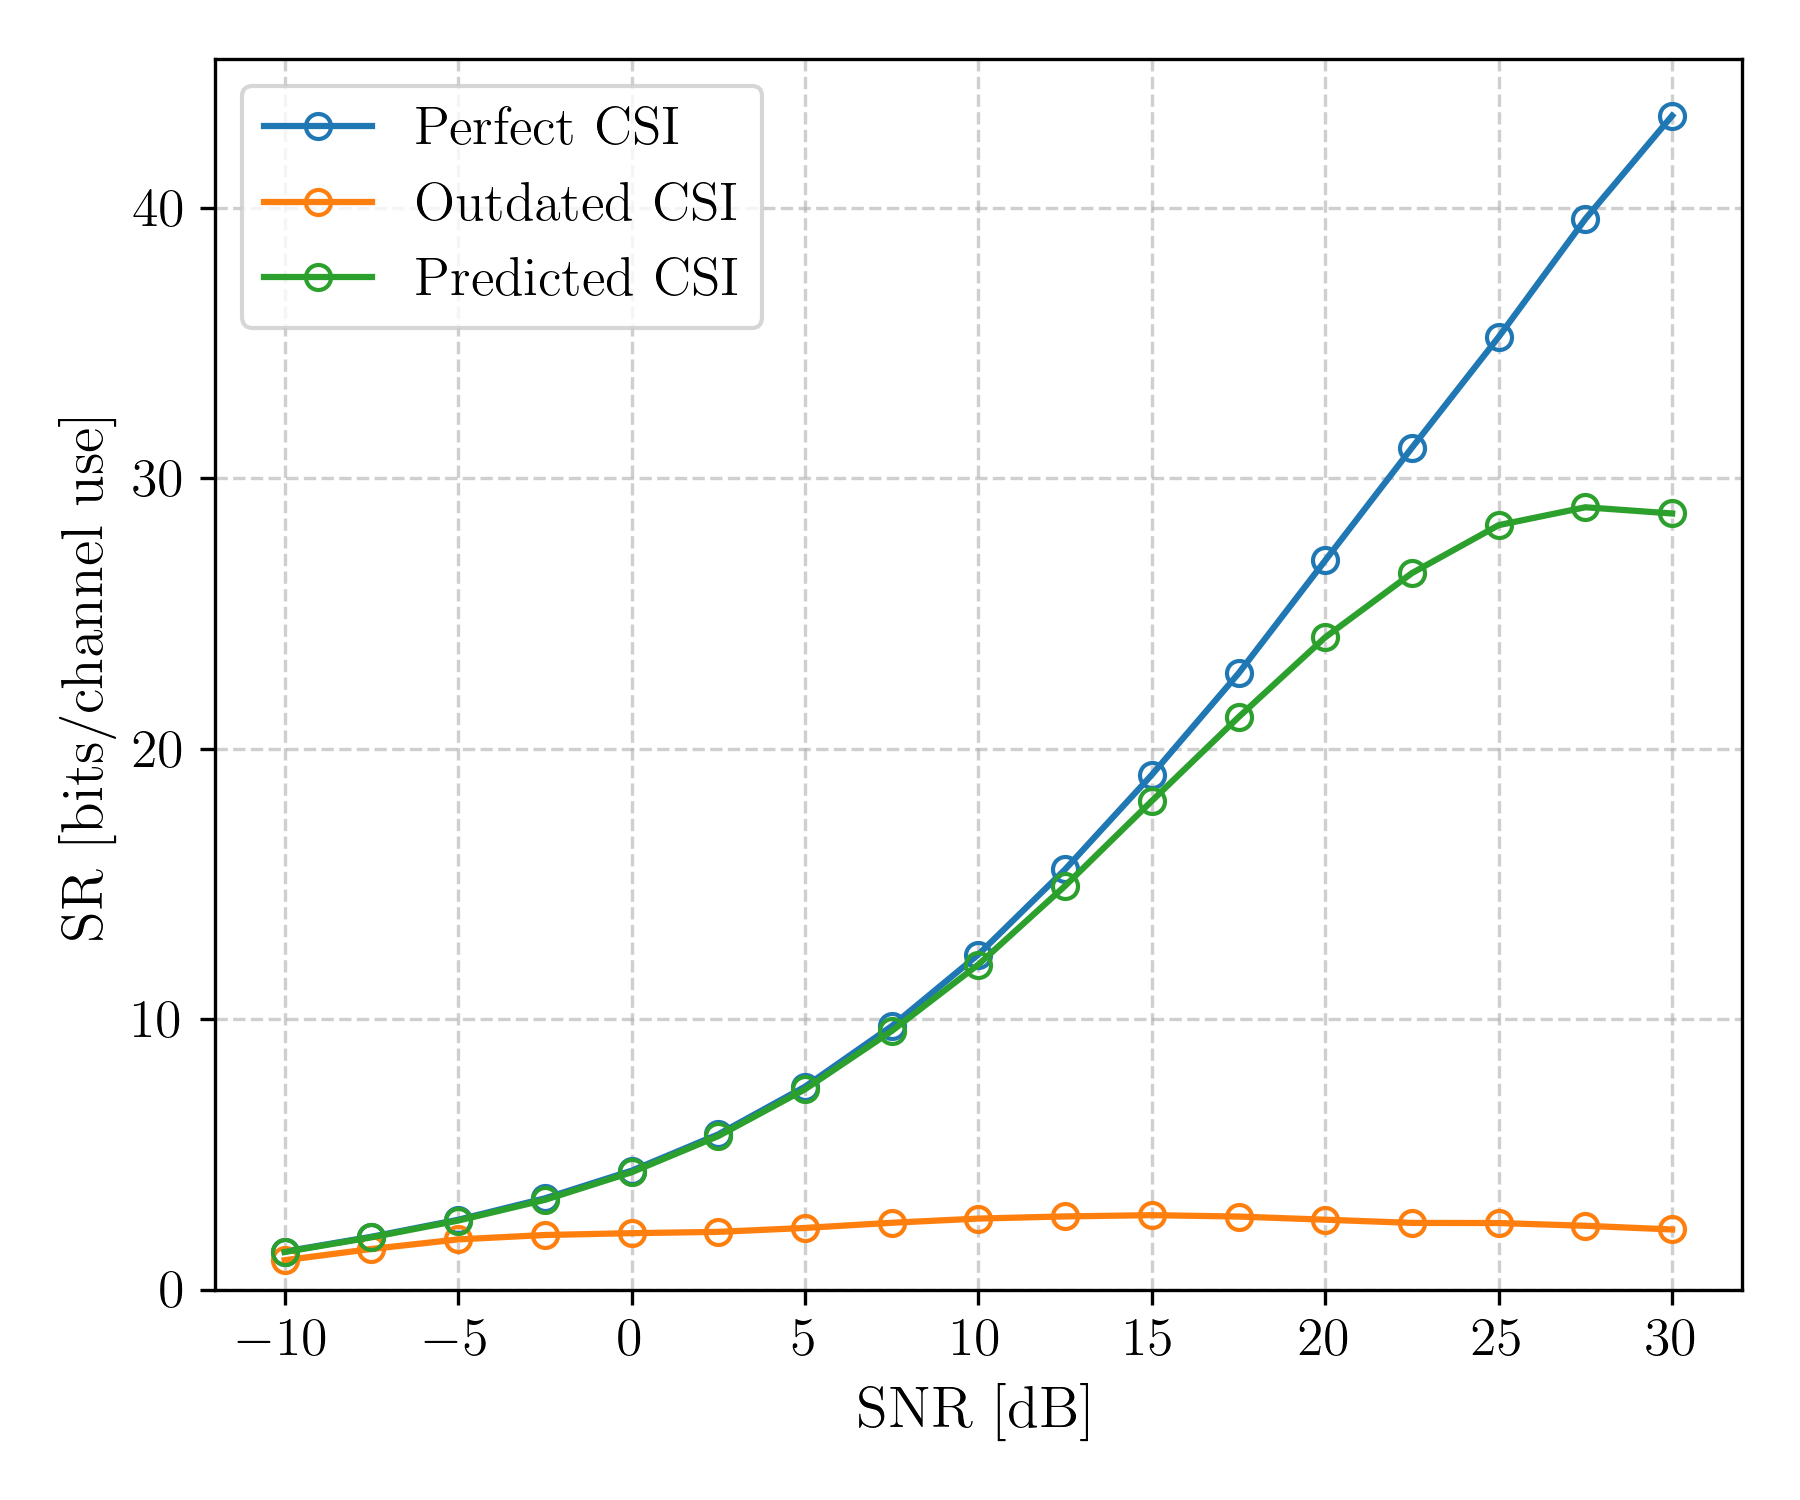
\includegraphics[width=\textwidth]{figures/satellite_communications_precoding/06_precoding_under_outdated_csi/rician_channel/impact_compensation/comparisons/wmmse/5on4.png}
                \caption{$\tau_{\mathrm{CSI}} = \frac{5}{4} T_c$}
            \end{subfigure}
            \hfill
            \begin{subfigure}{0.245\textwidth}
                \centering
                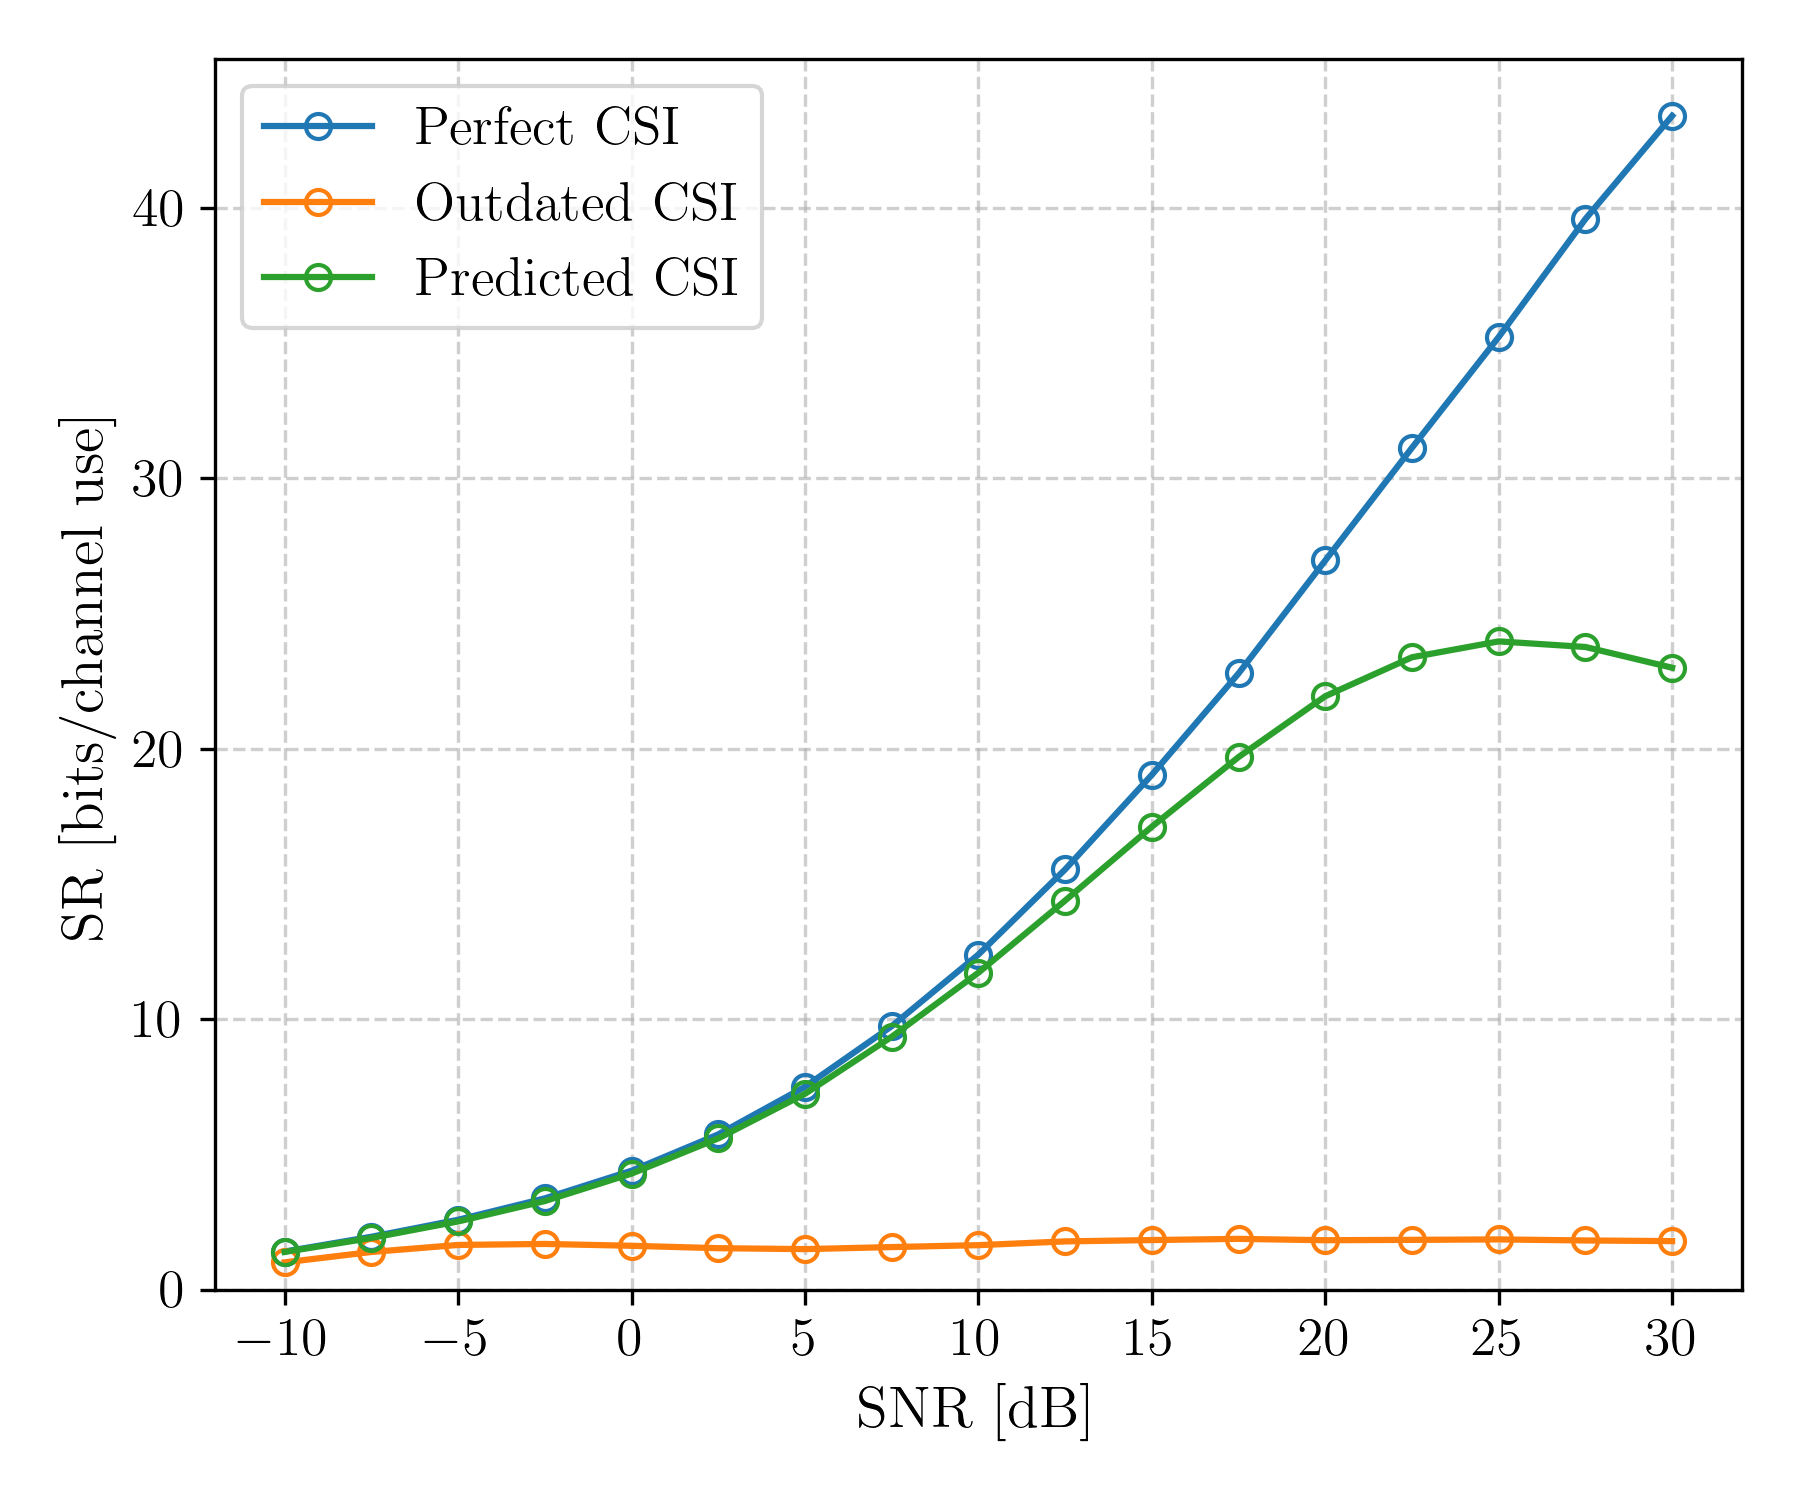
\includegraphics[width=\textwidth]{figures/satellite_communications_precoding/06_precoding_under_outdated_csi/rician_channel/impact_compensation/comparisons/wmmse/6on4.png}
                \caption{$\tau_{\mathrm{CSI}} = \frac{6}{4} T_c$}
            \end{subfigure}
            \hfill
            \begin{subfigure}{0.245\textwidth}
                \centering
                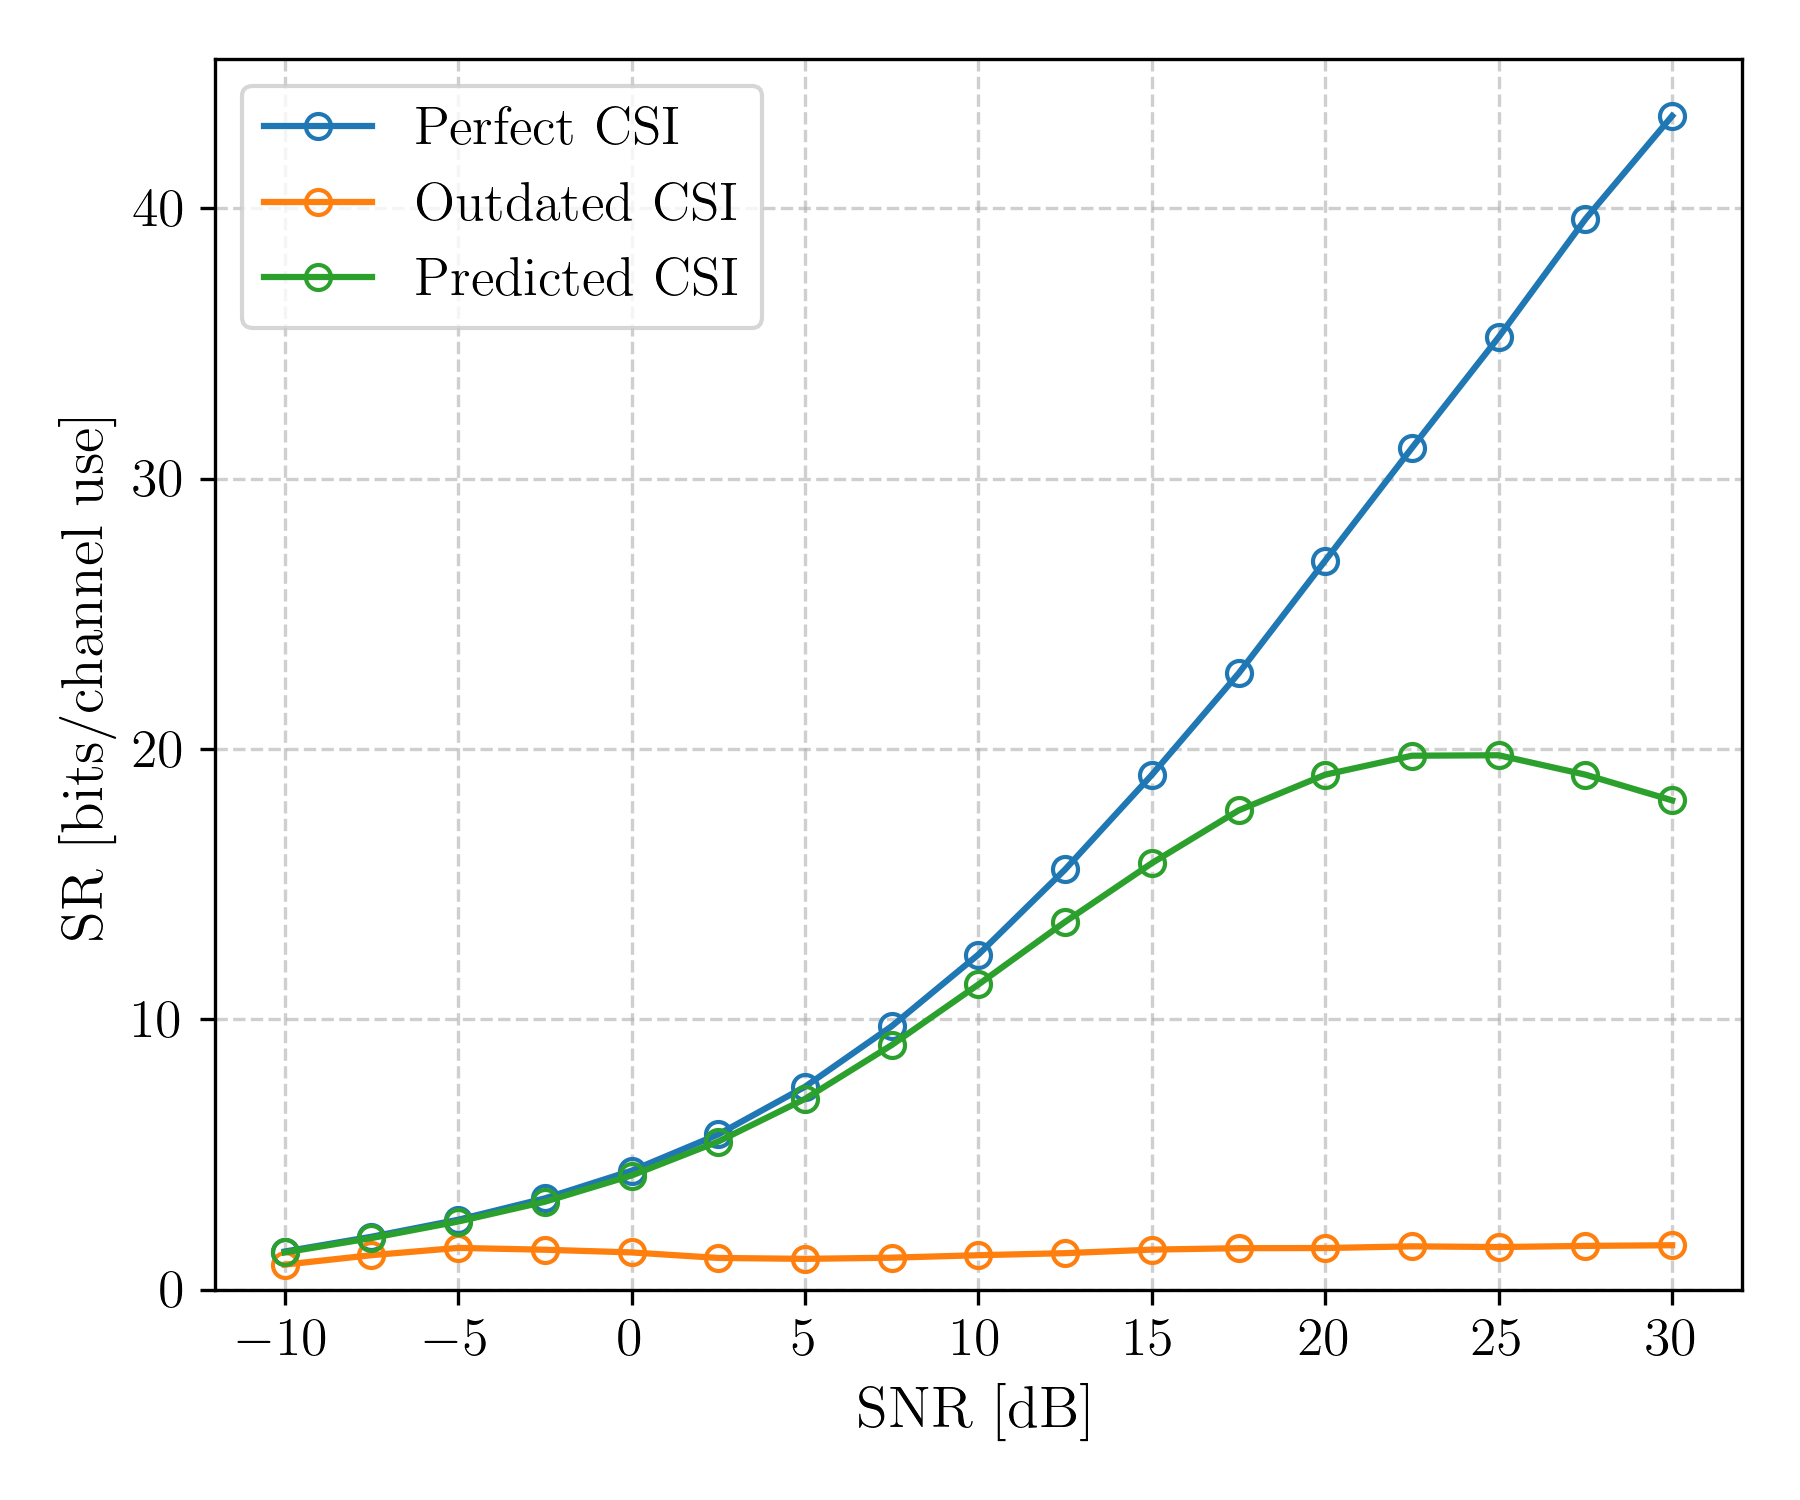
\includegraphics[width=\textwidth]{figures/satellite_communications_precoding/06_precoding_under_outdated_csi/rician_channel/impact_compensation/comparisons/wmmse/7on4.png}
                \caption{$\tau_{\mathrm{CSI}} = \frac{7}{4} T_c$}
            \end{subfigure}
            \hfill
            \begin{subfigure}{0.245\textwidth}
                \centering
                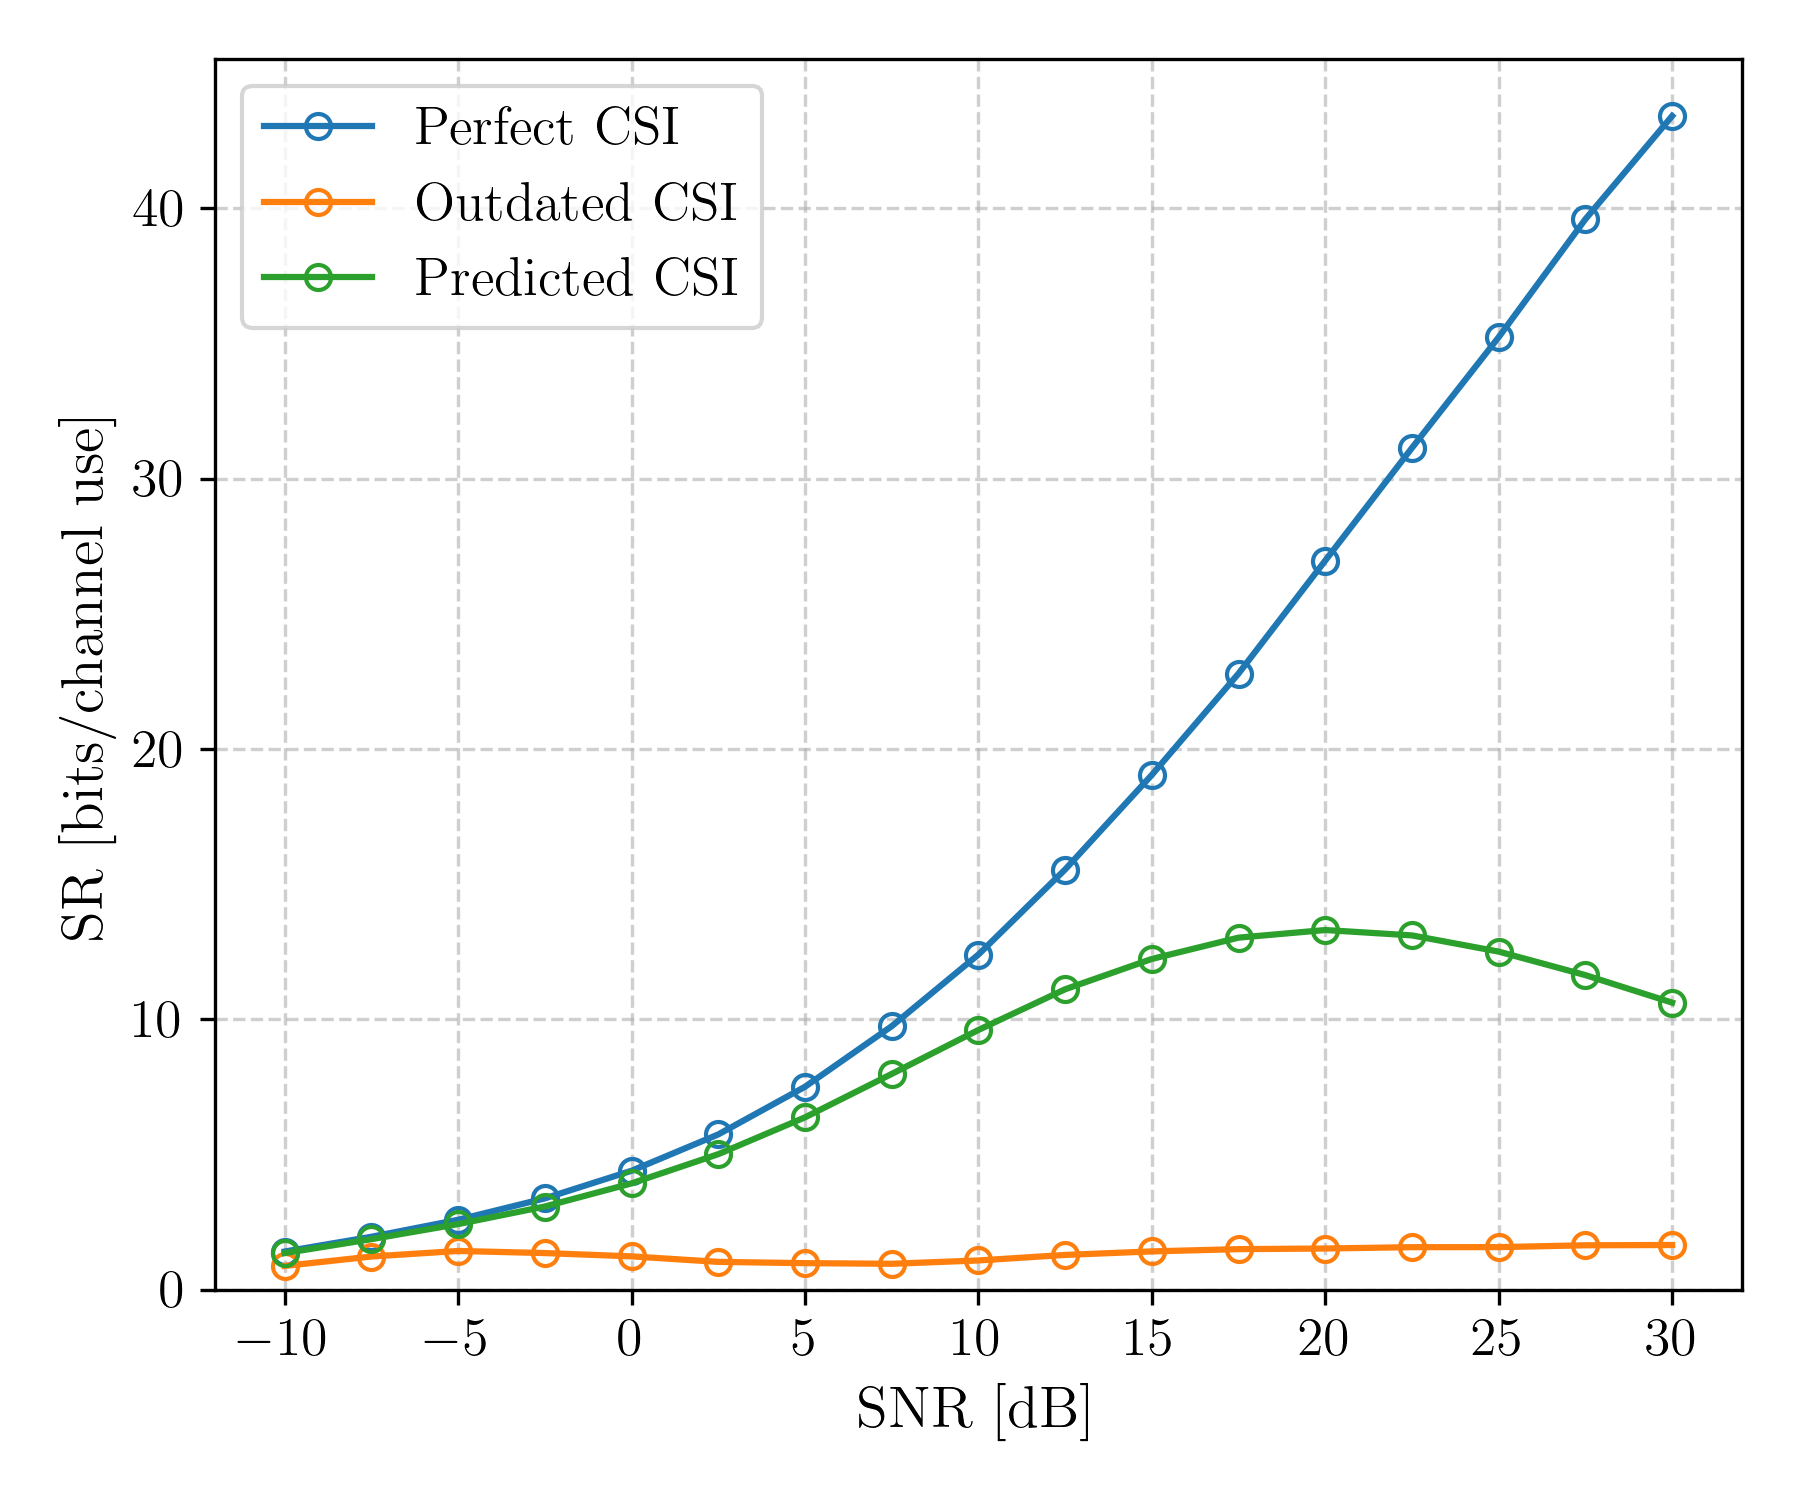
\includegraphics[width=\textwidth]{figures/satellite_communications_precoding/06_precoding_under_outdated_csi/rician_channel/impact_compensation/comparisons/wmmse/8on4.png}
                \caption{$\tau_{\mathrm{CSI}} = \frac{8}{4} T_c$}
            \end{subfigure}

        \end{minipage}
    }

    \caption[TO DO]{TODO}
    \label{fig:impact_compensation_achievable_rate_wmmse}
\end{figure}



\section{Evaluation on a More Realistic Channel}
\label{section:realistic_channel_evaluation}
% ==============================================
%    Evaluation on a More Realistic Channel
% ==============================================

\section{Conclusion}
\label{section:conclusion}
% ====================
%     Conclusion
% ====================
